%%%%%%%%%%%%%%%%%%%%%%%%%%%%%%%%%%%%%%%%%%%%%%%%%%%%%%%%%%%
\documentclass[xcolor=x11names,compress]{beamer}
%\documentclass[xcolor=x11names,compress, handhouts, aspectratio=169]{beamer}
%% General document
\usepackage{graphicx, subfig}
%% Beamer Layout
\useoutertheme[subsection=false,shadow]{miniframes}
\useinnertheme{default}
\usefonttheme{serif}
\usepackage{palatino}

%%%%%%% Mes Packages %%%%%%%%%%%%%%%%
%\usepackage[french]{babel}
\usepackage[T1]{fontenc}
\usepackage{color}
\usepackage{xcolor}
\usepackage{dsfont} % Pour indicatrice
\usepackage{url}
\usepackage{multirow}
\usepackage[normalem]{ulem}   % For strike out text

% Natbib for clean bibliography
\usepackage[comma,authoryear]{natbib}

%remove the icon
\setbeamertemplate{bibliography item}{}

%remove line breaks
\setbeamertemplate{bibliography entry title}{}
\setbeamertemplate{bibliography entry location}{}
\setbeamertemplate{bibliography entry note}{}

%% ------ MEs couleurs --------
\definecolor{vert}{rgb}{0.1,0.7,0.2}
\definecolor{brique}{rgb}{0.7,0.16,0.16}
\definecolor{gris}{rgb}{0.7, 0.75, 0.71}
\definecolor{twitterblue}{rgb}{0, 0.42, 0.58}
\definecolor{airforceblue}{rgb}{0.36, 0.54, 0.66}
\definecolor{siap}{RGB}{3,133, 200}


%%%%%%%%%%%%%%%%% BEAMER PACKAGE %%%%%%%

\setbeamercolor{itemize item}{fg=siap}
%\setbeamercolor{itemize subitem}{fg=blue}
%\setbeamercolor{itemize subsubitem}{fg=cyan}

\setbeamerfont{title like}{shape=\scshape}
\setbeamerfont{frametitle}{shape=\scshape}

\setbeamercolor*{lower separation line head}{bg=DeepSkyBlue4}
\setbeamercolor*{normal text}{fg=black,bg=white}
\setbeamercolor*{alerted text}{fg=siap}
\setbeamercolor*{example text}{fg=black}
\setbeamercolor*{structure}{fg=black}
\setbeamercolor*{palette tertiary}{fg=black,bg=black!10}
\setbeamercolor*{palette quaternary}{fg=black,bg=black!10}

% Set the header color to SIAP's color
\setbeamercolor*{frametitle}{fg=siap}

%remove navigation symbols
\setbeamertemplate{navigation symbols}{}

\renewcommand{\(}{\begin{columns}}
\renewcommand{\)}{\end{columns}}
\newcommand{\<}[1]{\begin{column}{#1}}
\renewcommand{\>}{\end{column}}

%% Add footer with logo
\setbeamertemplate{footline}{%
  \begin{beamercolorbox}[wd=\paperwidth,ht=2.5ex,dp=1.125ex,%
    leftskip=.3cm,rightskip=.3cm plus1fil]{author in head/foot}
    
\includegraphics[height=5ex]{SIAP-ESCAP-Logo.png}\hfill
    \insertshortauthor\hfill\insertshorttitle\hfill  \textcolor{siap}{\textit{\insertframenumber}}
  \end{beamercolorbox}%
}

% Path for the graphs
\graphicspath{
{Graphics/}
%{c:/Chris/UN-ESCAP/SIAP-E-learning/Resources/OpenScience/}
%{c:/Chris/Visualisation/Presentations/Graphics/}
%{c:/Chris/Visualisation/Presentations/Graphics/SIAP/}
%{c:/Chris/Visualisation/Presentations/Graphics/Lies/}
%{c:/Chris/Visualisation/Presentations/Graphics/Maps/}
%{c:/Chris/Visualisation/Presentations/Graphics/RGenerated/}
%{c:/Chris/Visualisation/Presentations/Graphics/Logos/}
%{c:/Gitmain/MLCourse/UNML/Module0/M0_files/figure-html/}
%{c:/Chris/UN-ESCAP/MyCourses2022/MLOS2022/Slides/Graphics/}
%{c:/Chris/UN-ESCAP/MyCourses2023/RAP/Slides/Graphics/}
%{c:/GitMain/RAP/RAP-Course/images/}
%{c:/Chris/UN-ESCAP/MyCourses2022/MLOS2022/Slides/Graphics/}
%% Path for specific graphs created
% {../R-Codes/JobSatisfaction_files/figure-latex/}
% {../R-Codes/Unused_files/figure-latex/}
 }


\title{\textcolor{siap}{Training on Web Scraping Prices for CPI \\ \vspace{0.5cm} }}

\subtitle{\textcolor{brique}{\Large{ Reproducible Analytical Pipelines}}}
\author{Christophe Bontemps \& Serge Goussev }
\institute{ 
\includegraphics[height=9ex]{SIAP-ESCAP-Logo.png} \hspace{1cm} 
\includegraphics[height=10ex]{StatCanada-Logo.jpg}}
\date{}

\begin{document}

\section{Motivation}

\begin{frame}
  \titlepage
\end{frame}

\begin{frame}{Fundamental Principles of Official Statistics}
  \begin{columns}[T]
    \begin{column}{0.6\textwidth}
      \begin{itemize}[<+->]
        \item Clear mention of the \textbf{processes} used to produce statistics
        \item \emph{To retain trust in official statistics, the \textbf{statistical agencies need to decide} according to strictly professional considerations, including scientific principles and professional ethics, \textbf{on the methods and procedures} for the collection, processing, storage and presentation of statistical data.}
      \item In short, \textbf{processes} are important! 
      \end{itemize}
    \end{column}
    \begin{column}{0.4\textwidth}
      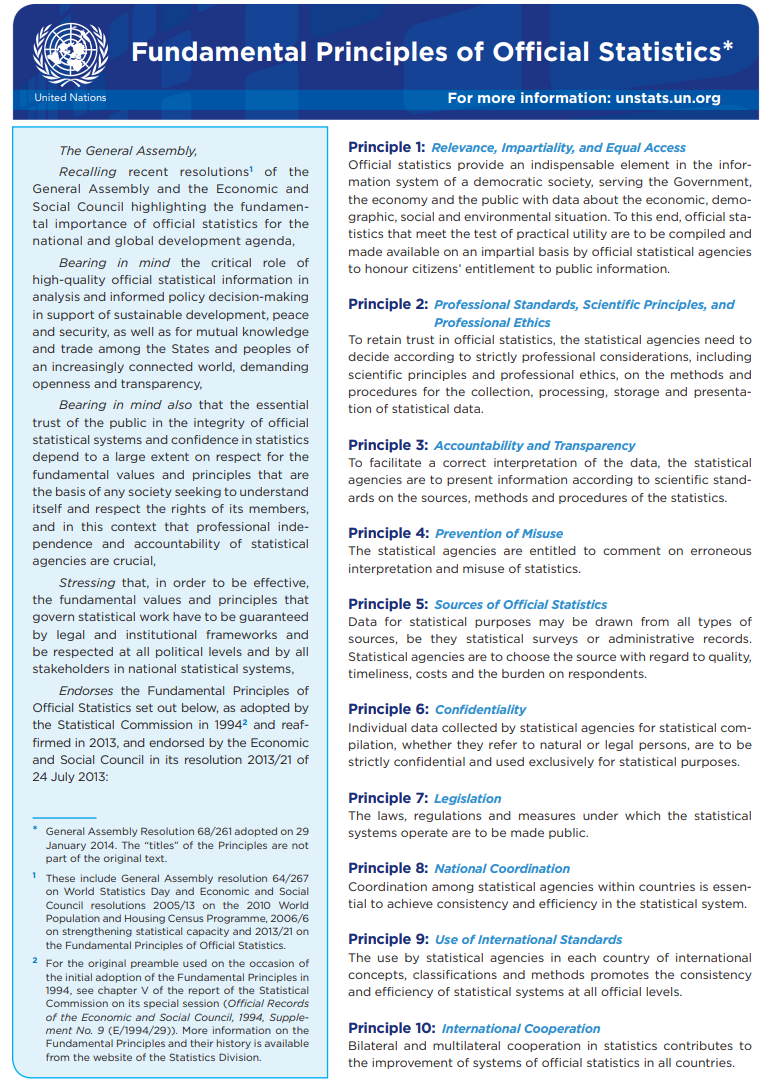
\includegraphics[width=\textwidth]{FundamentalPrinciplesOS.PNG}
    \end{column}
  \end{columns}
\end{frame}

\begin{frame}{Usual practice: Theory vs reality}
\begin{center}
  \begin{itemize}
        \only<1>{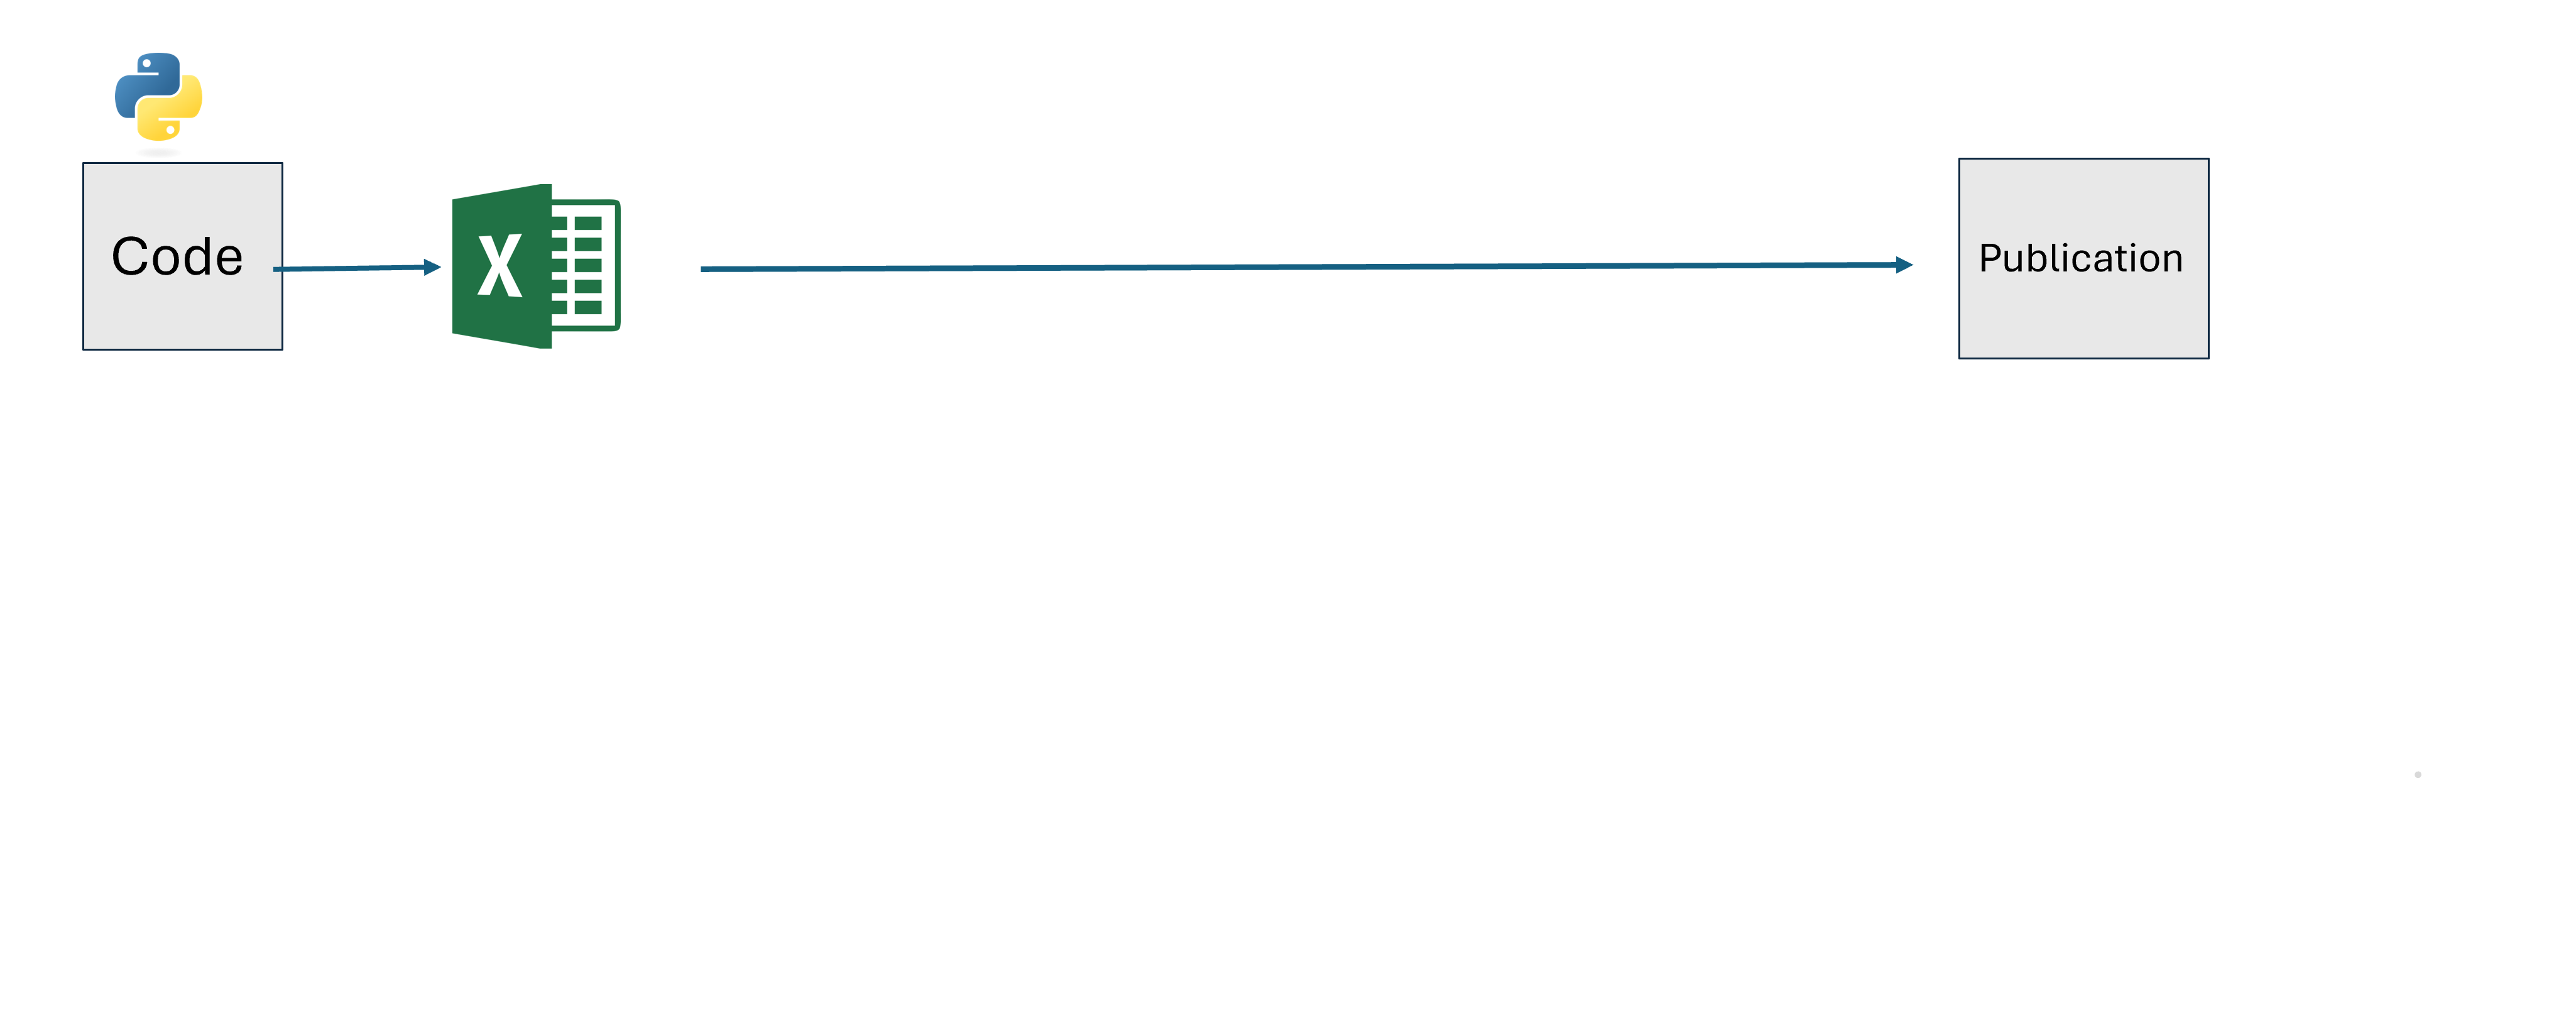
\includegraphics[width=0.8\textwidth]{Process1.png} \\ Comment 1}
        \only<2>{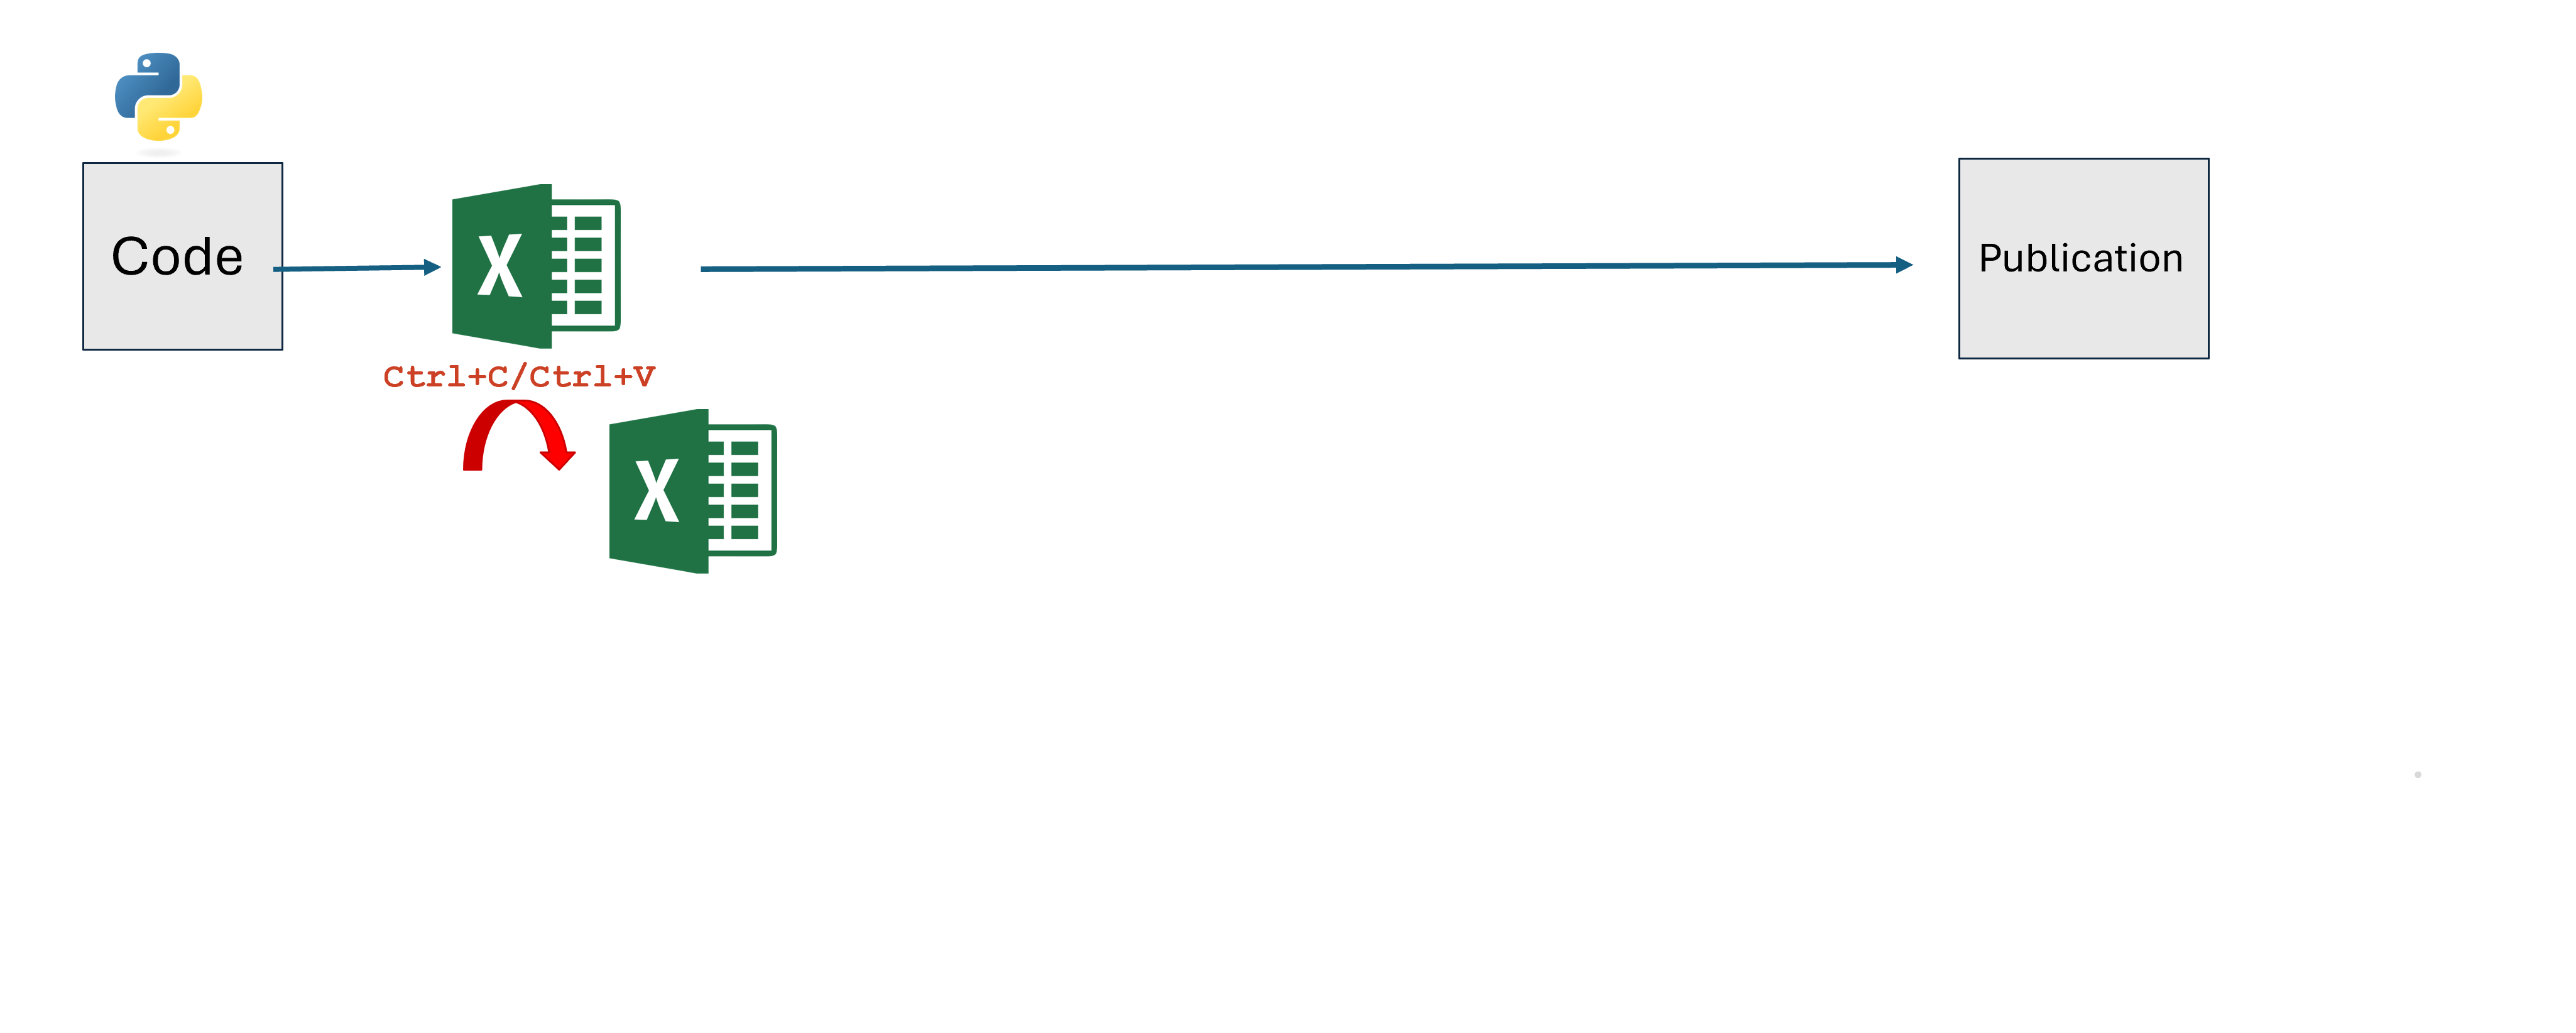
\includegraphics[width=0.8\textwidth]{Process2.png} \\ Comment 2}
        \only<3>{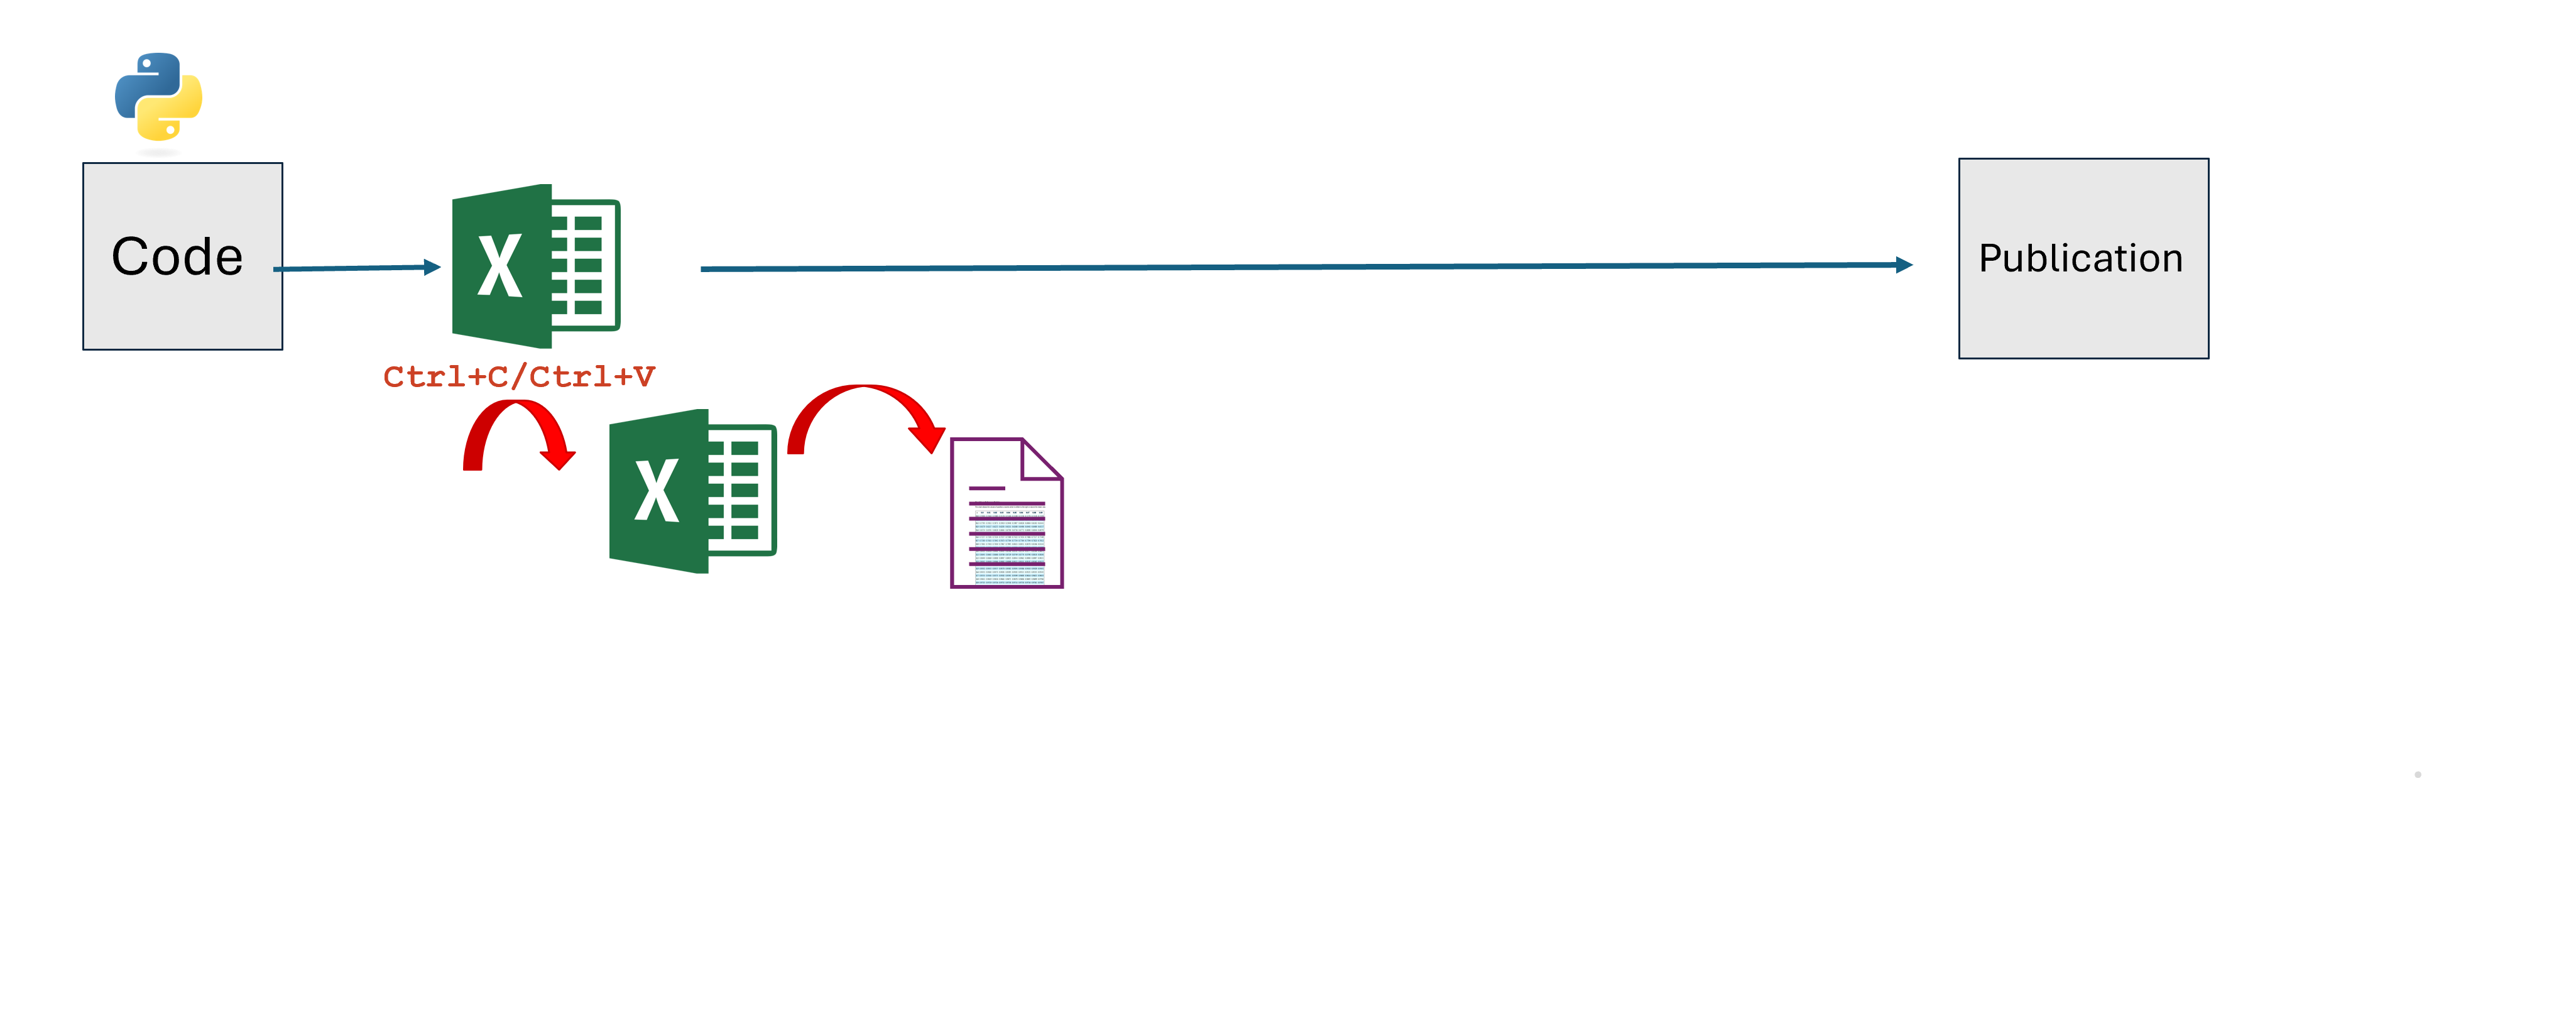
\includegraphics[width=0.8\textwidth]{Process3.png} \\ Comment 3}
        \only<4>{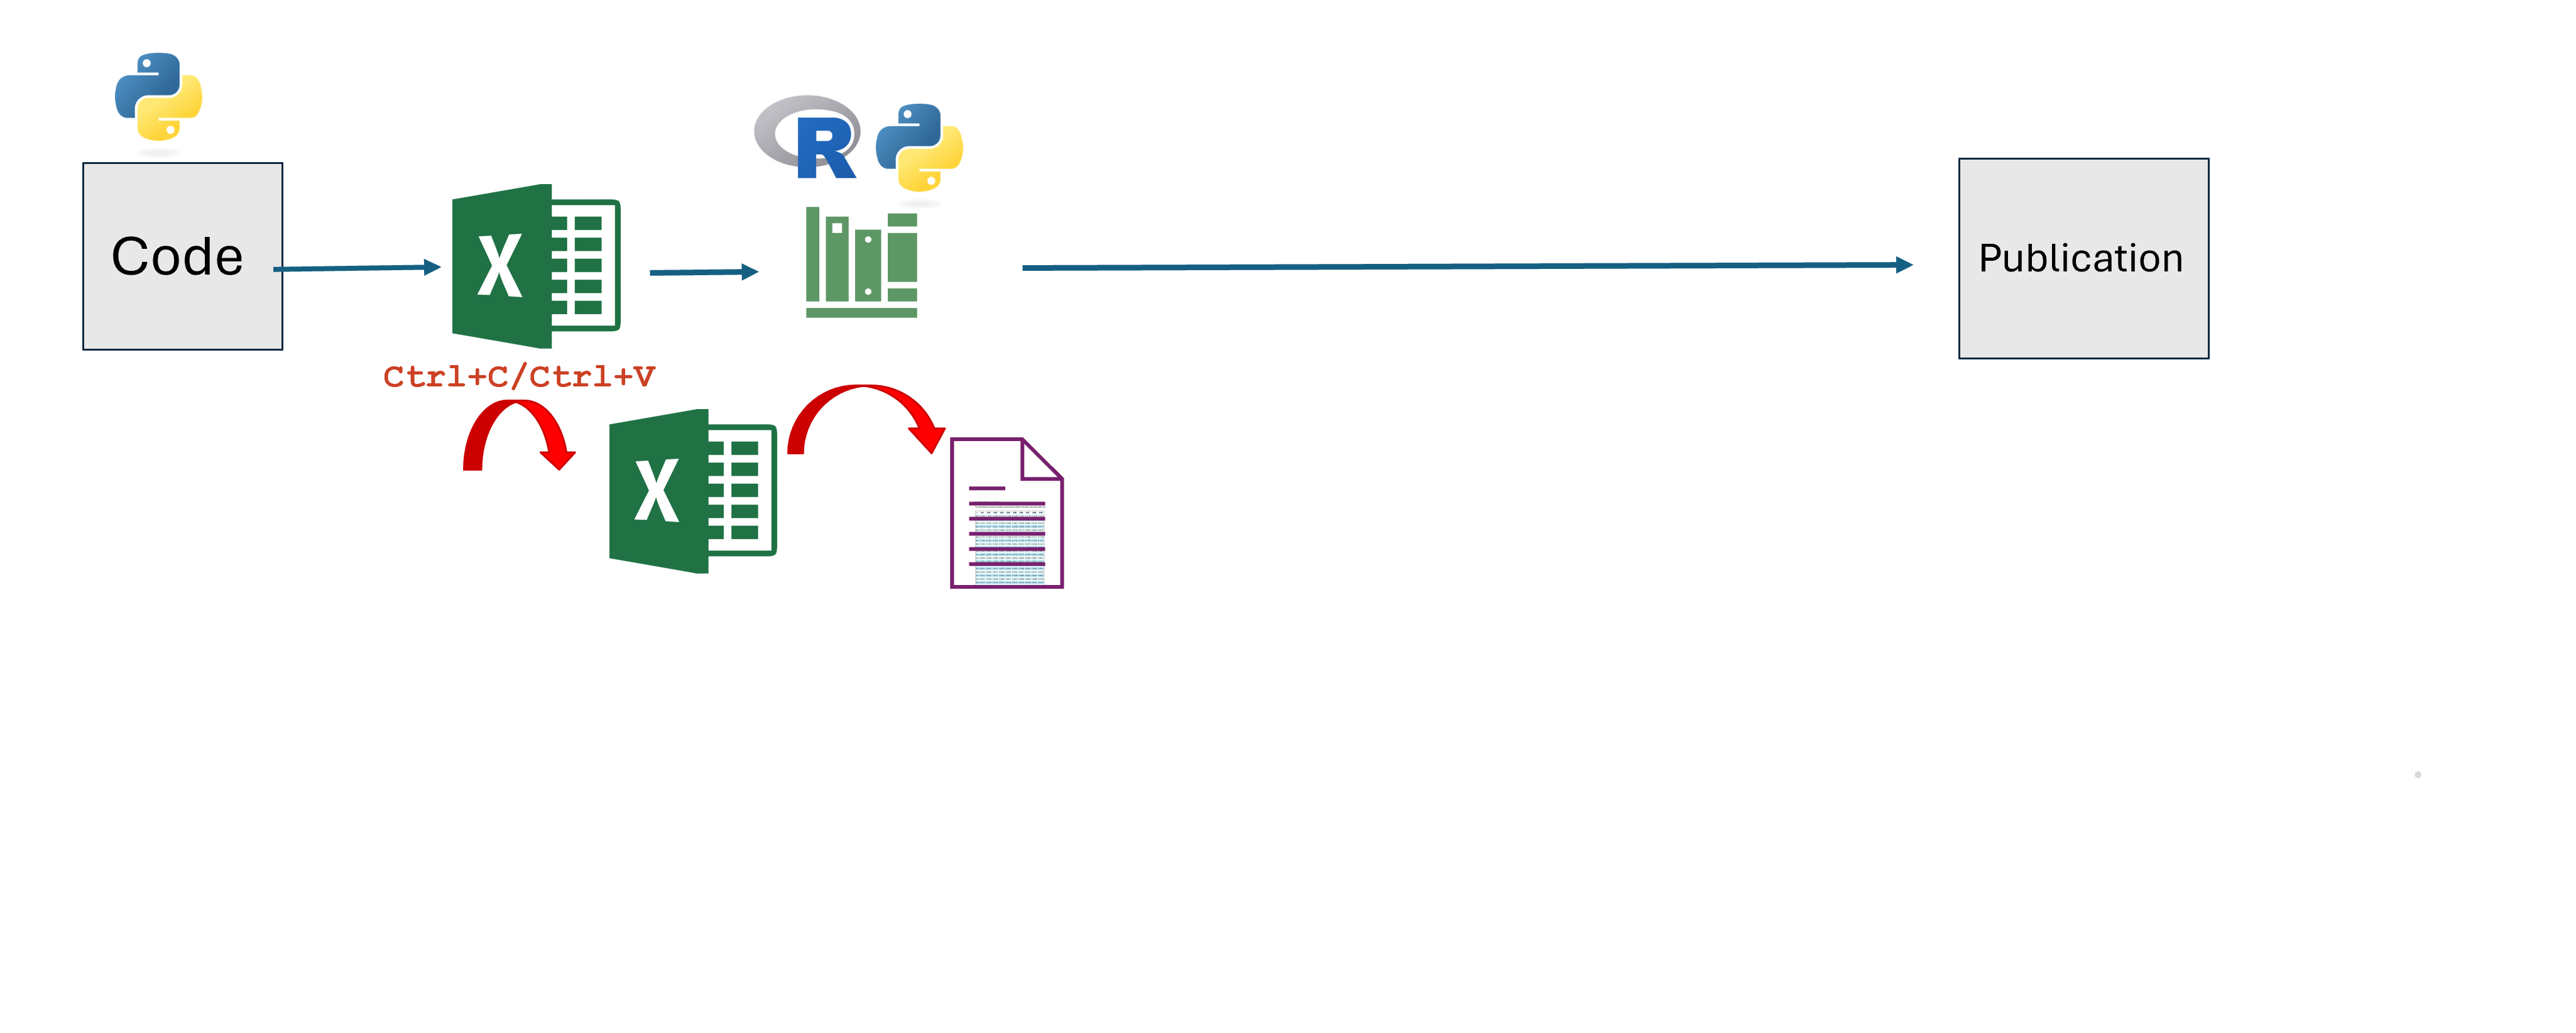
\includegraphics[width=0.8\textwidth]{Process4.png} \\ Comment 4}
        \only<5>{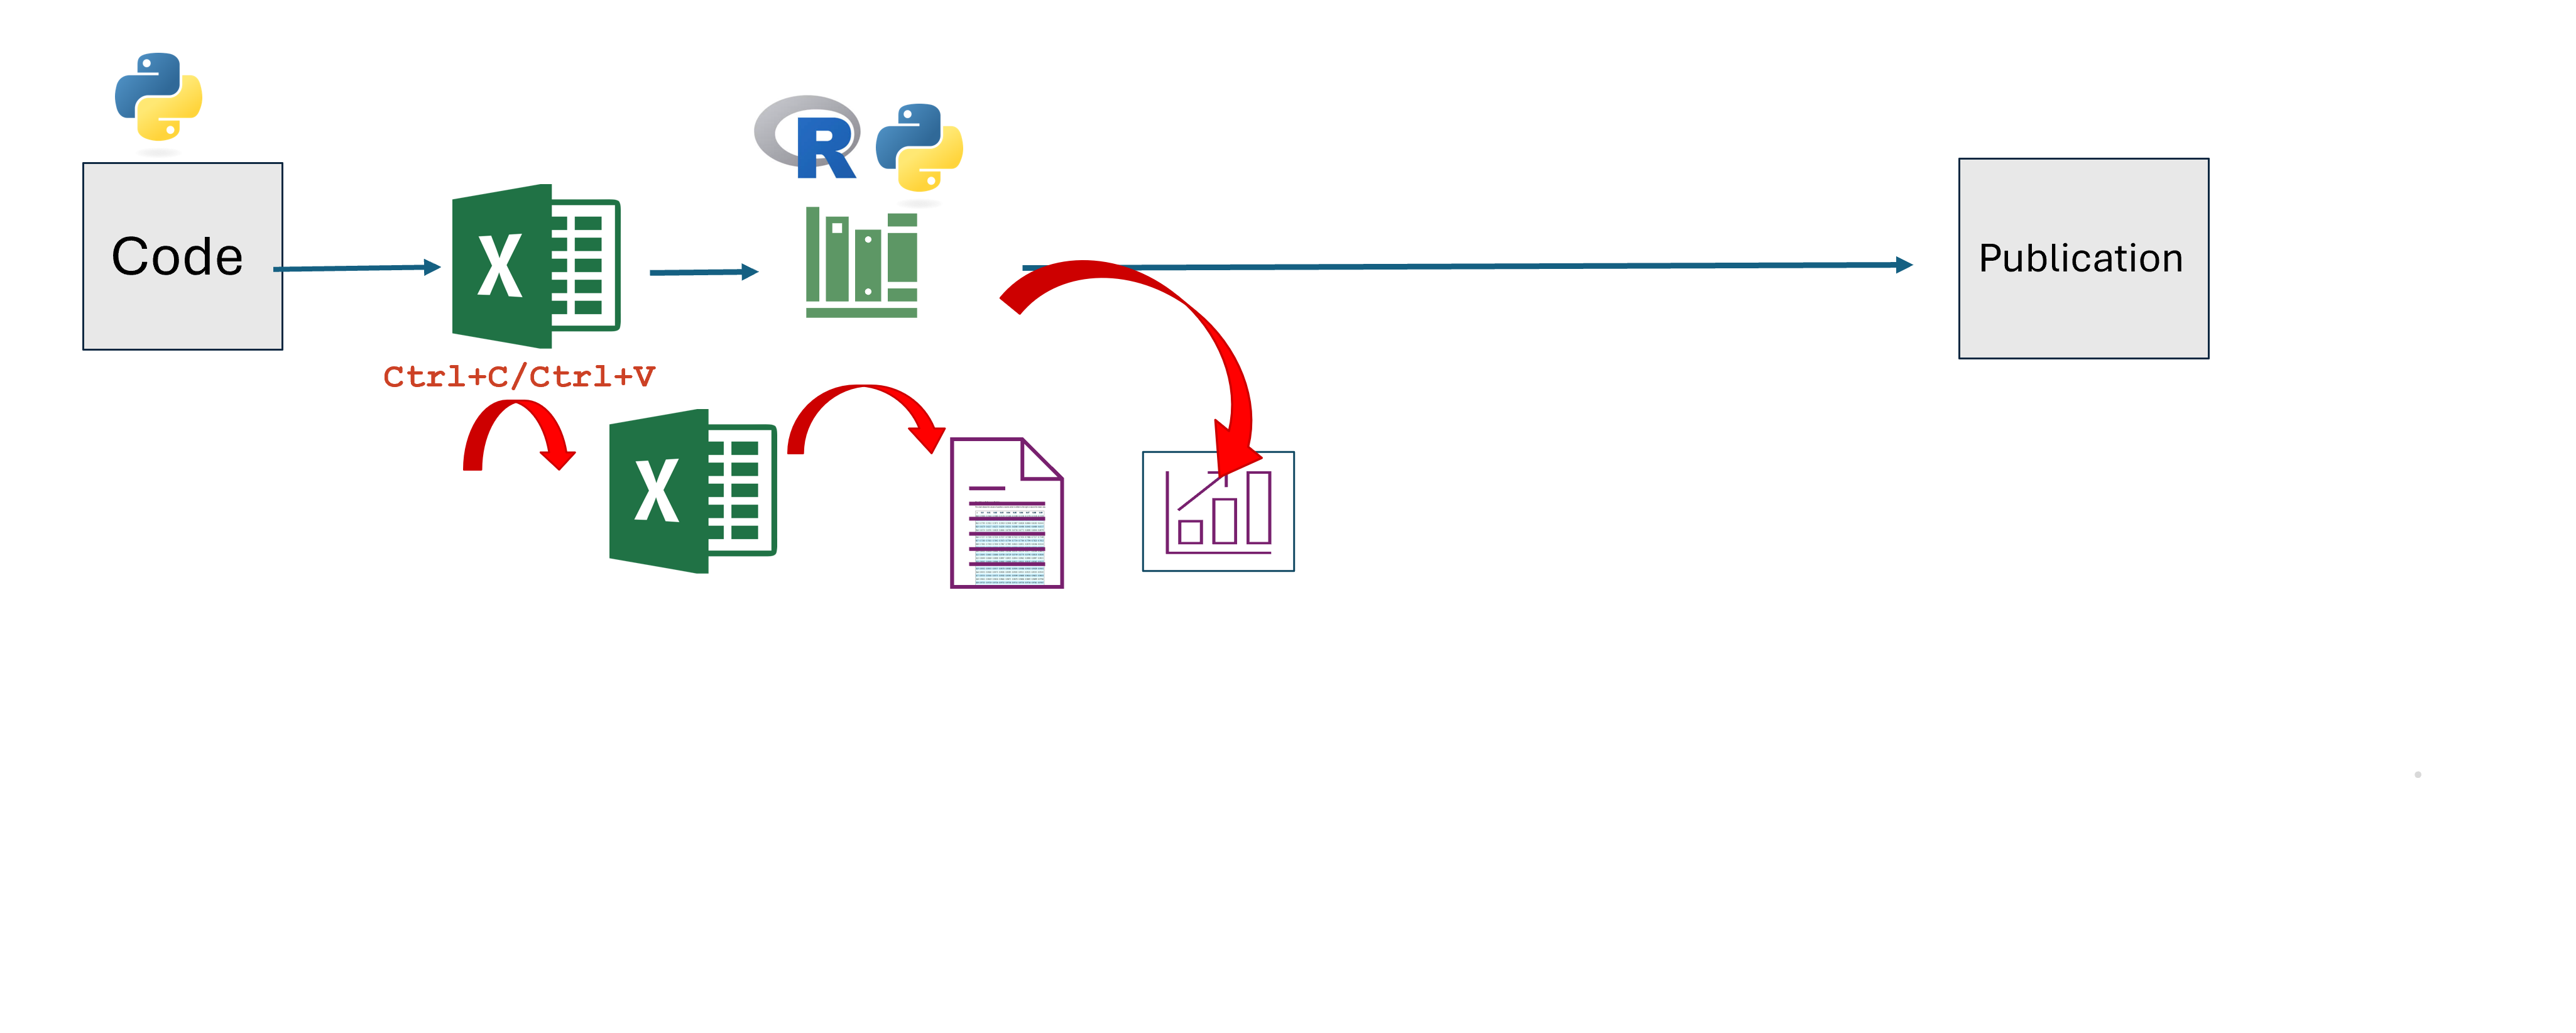
\includegraphics[width=0.8\textwidth]{Process5.png} \\ Comment 5}
        \only<6>{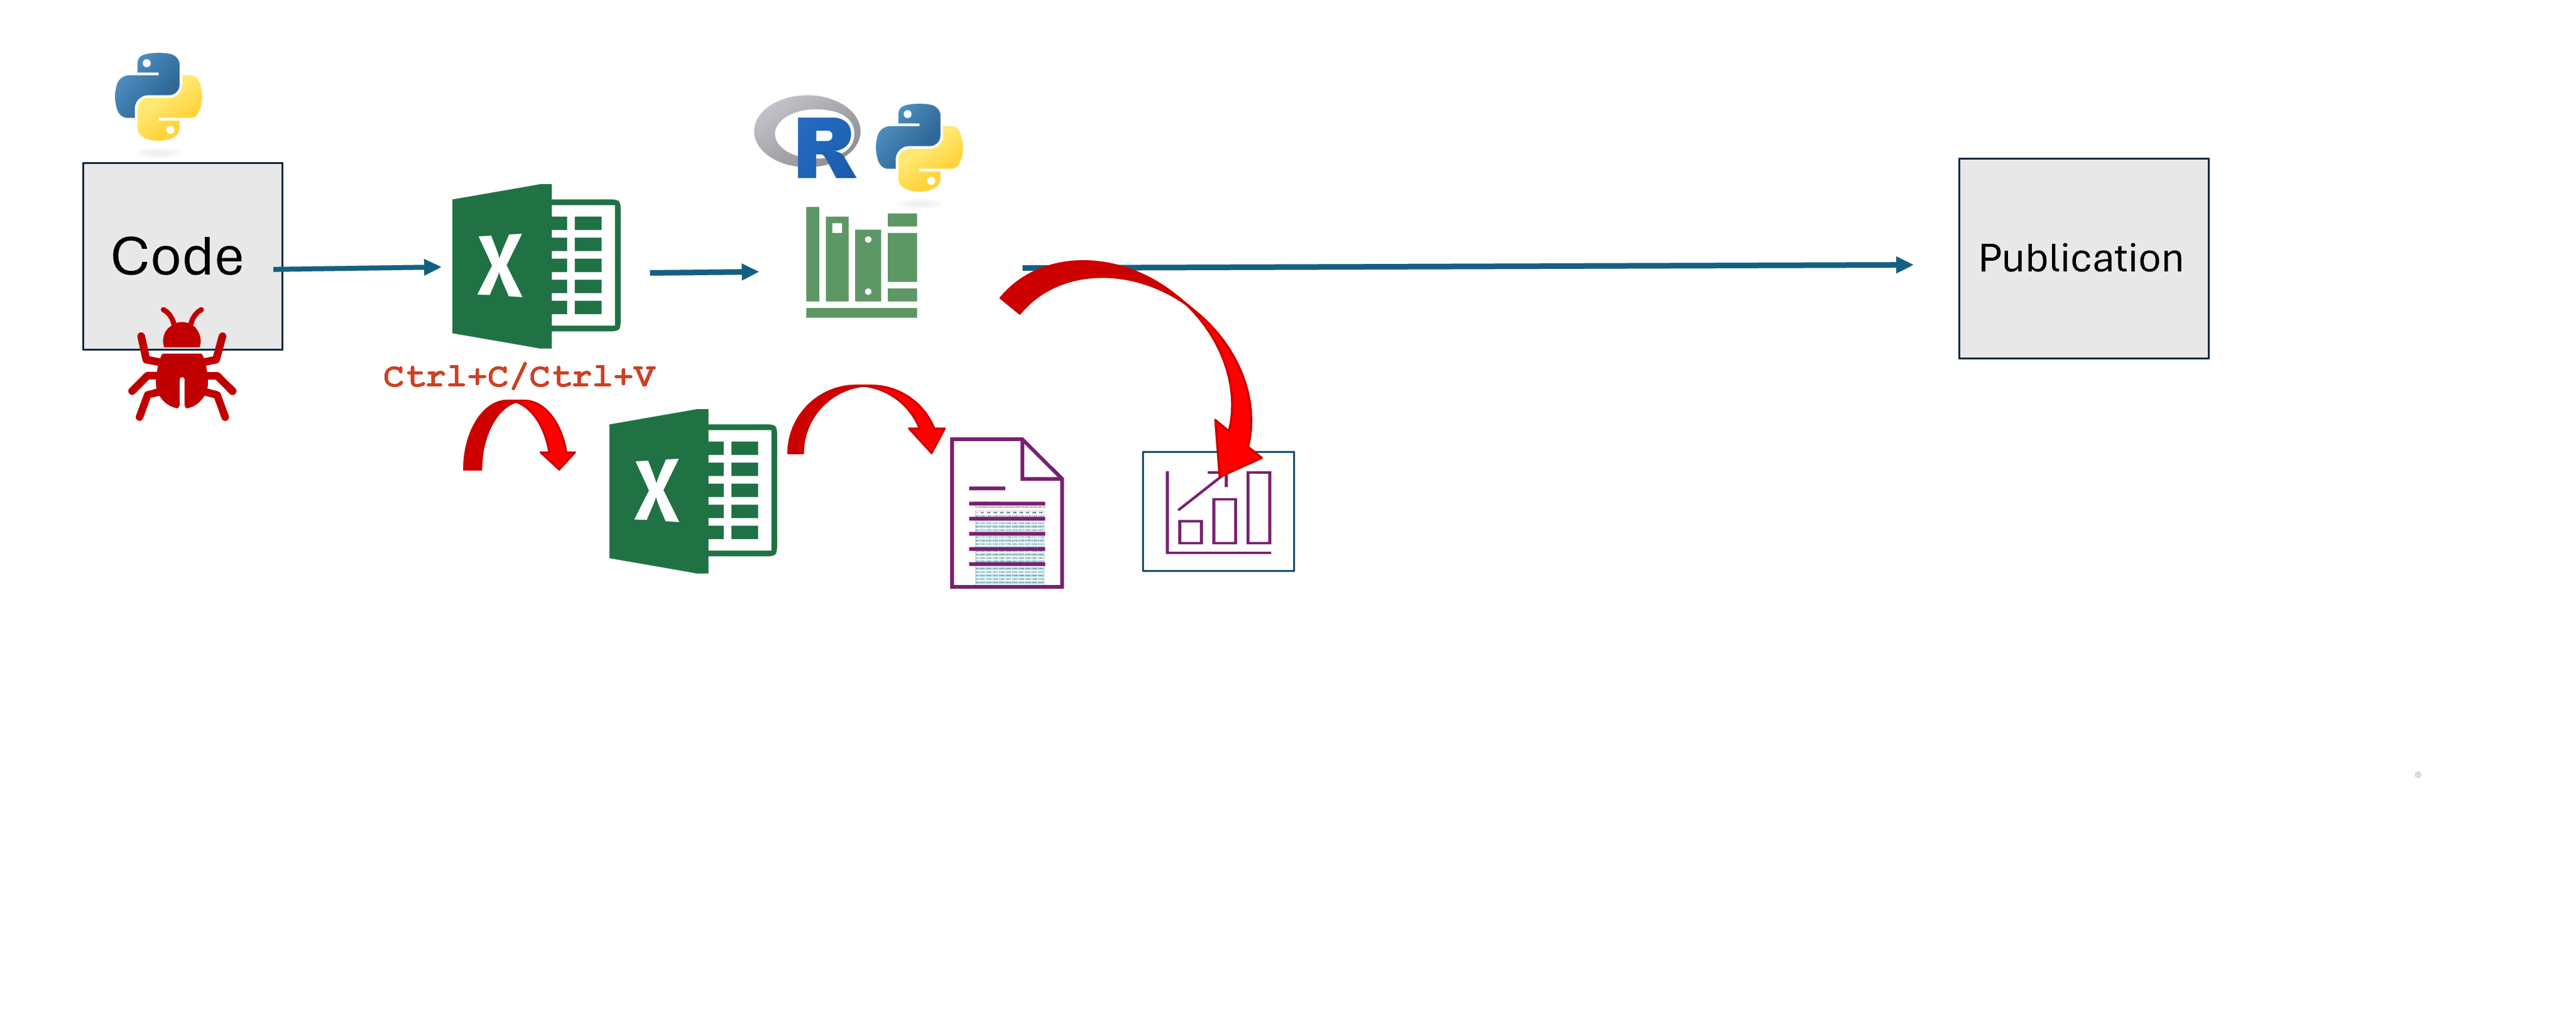
\includegraphics[width=0.8\textwidth]{Process6.png} \\ Comment 6}
        \only<7>{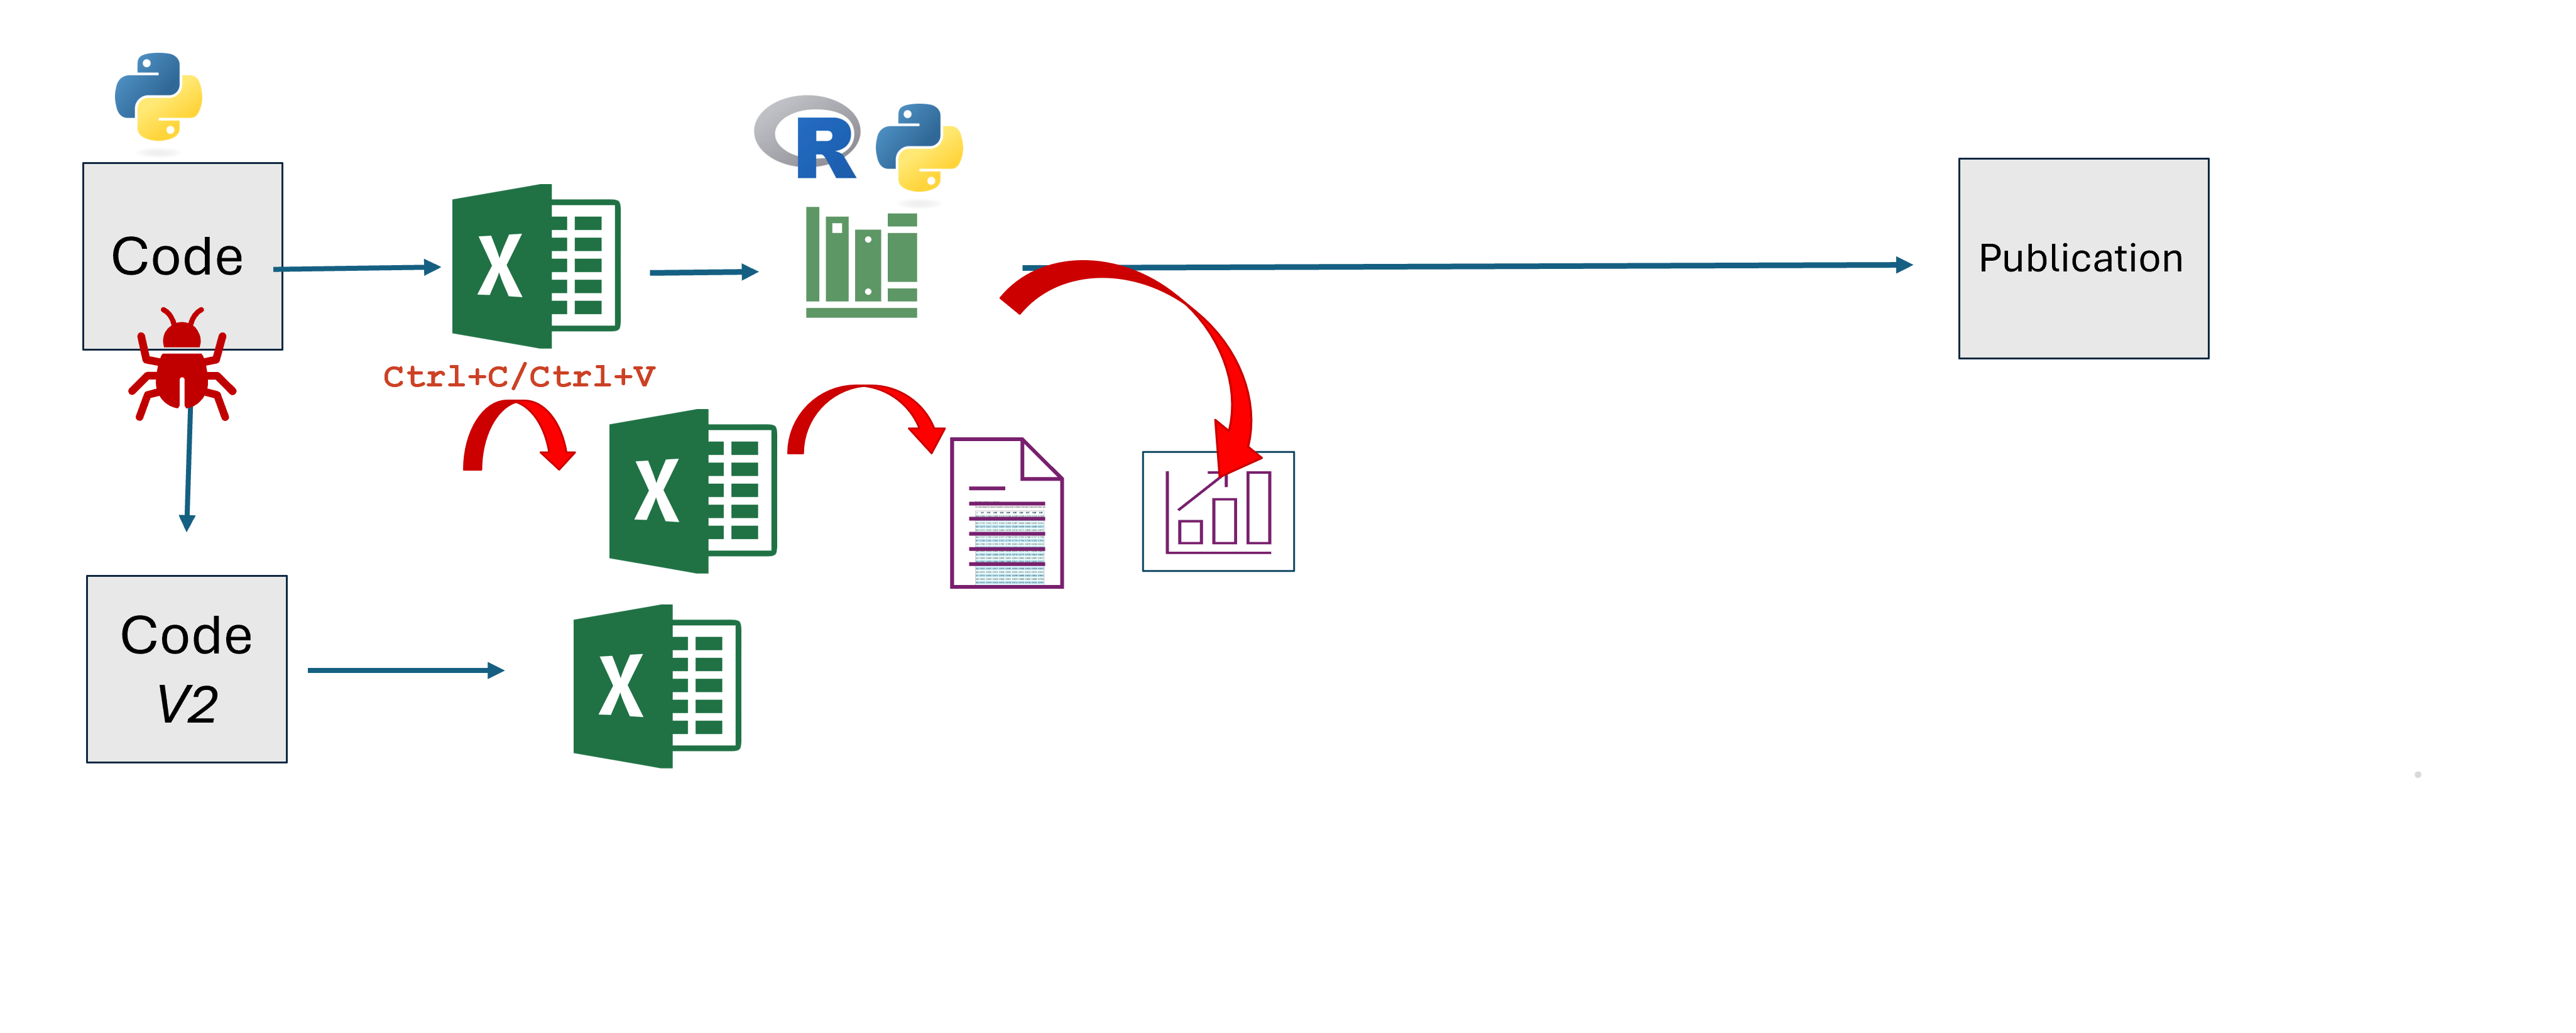
\includegraphics[width=0.8\textwidth]{Process7.png} \\ Comment 7}
        \only<8>{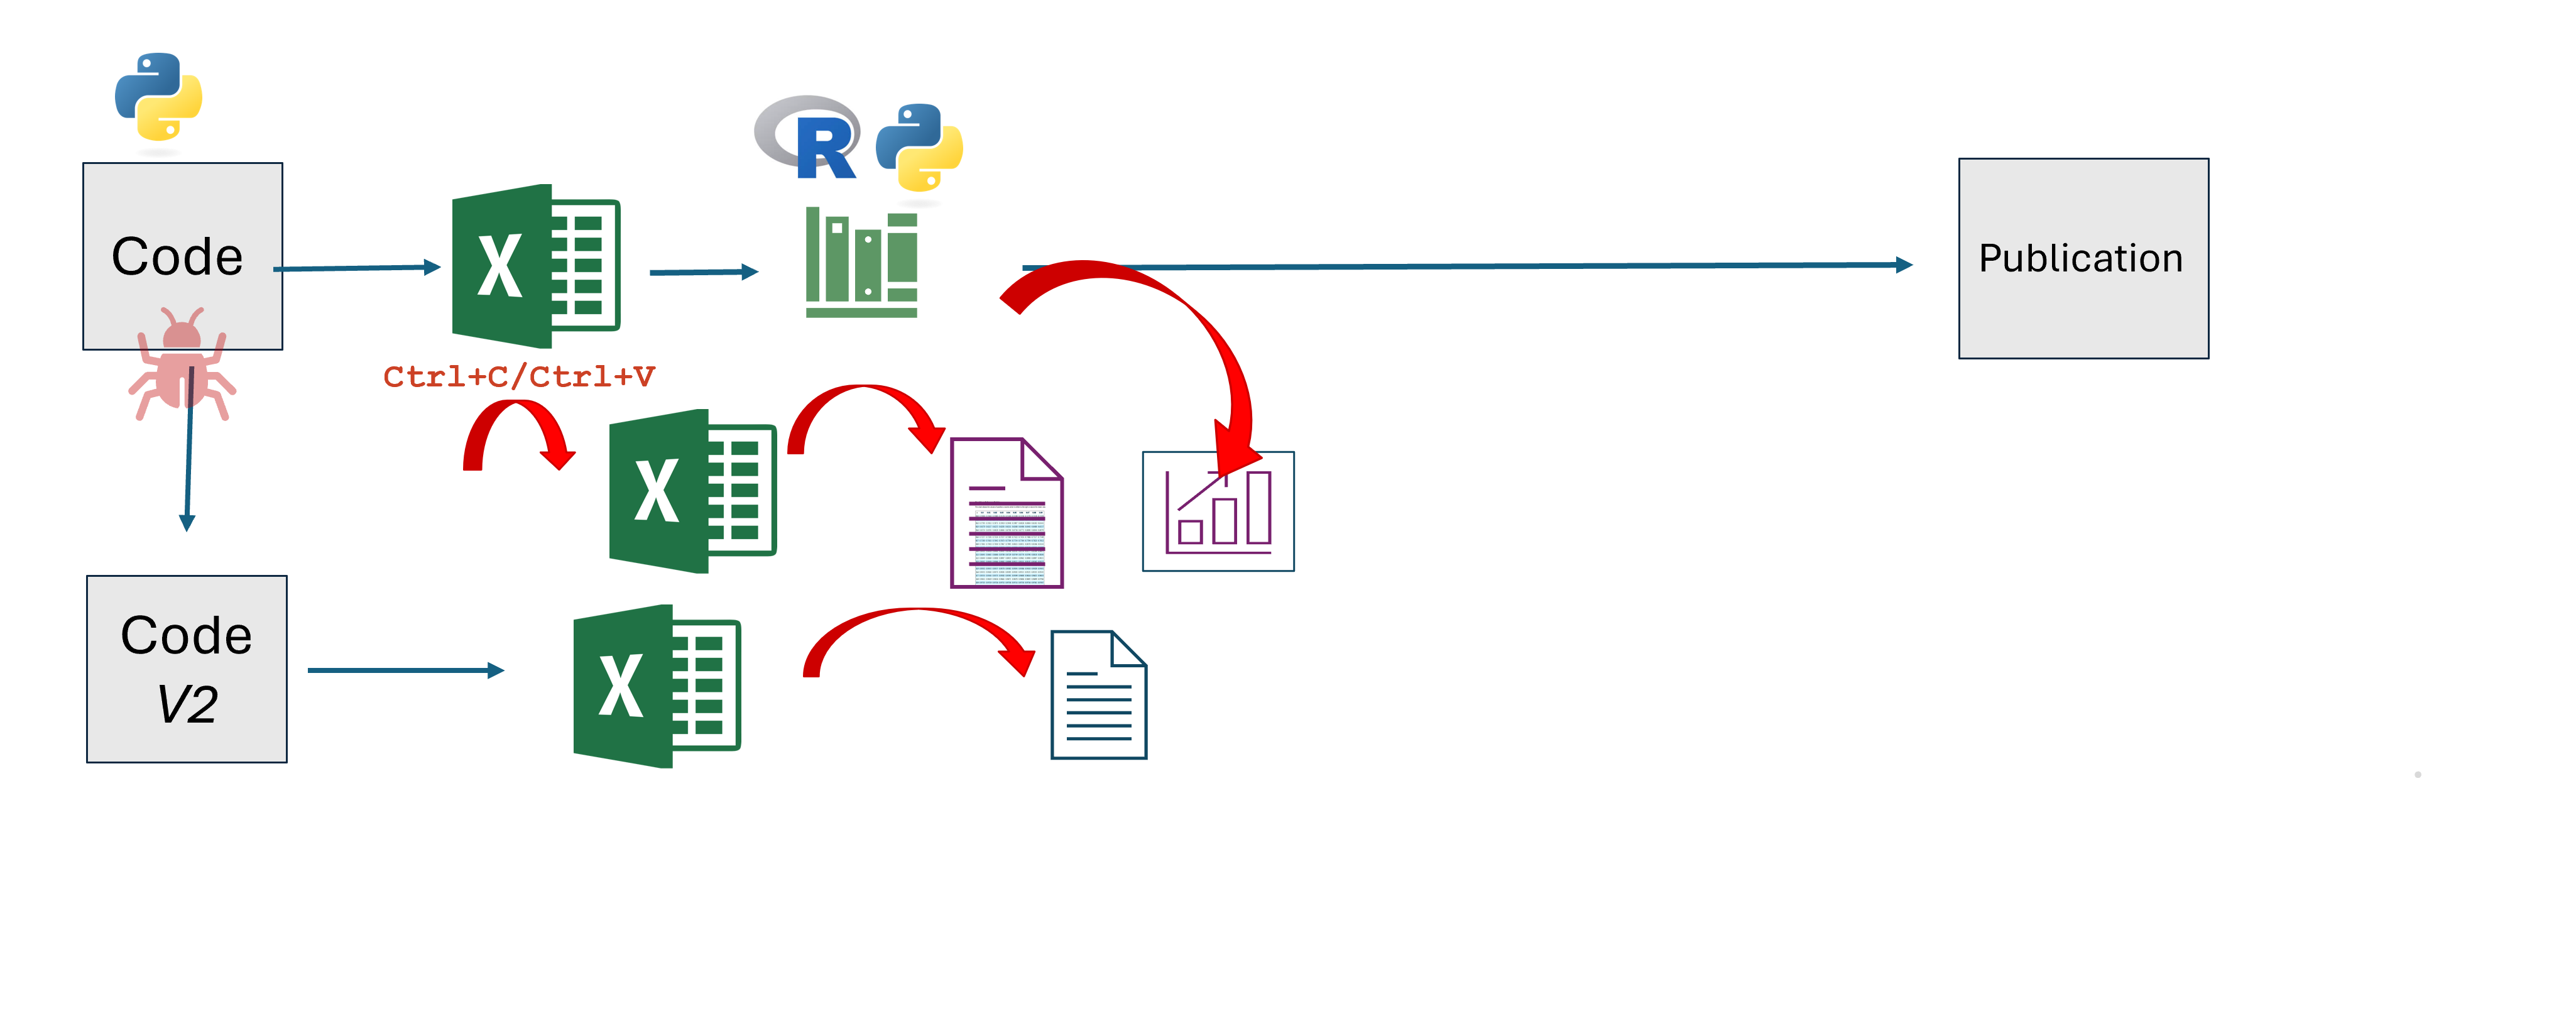
\includegraphics[width=0.8\textwidth]{Process8.png} \\ Comment 8}
        \only<9>{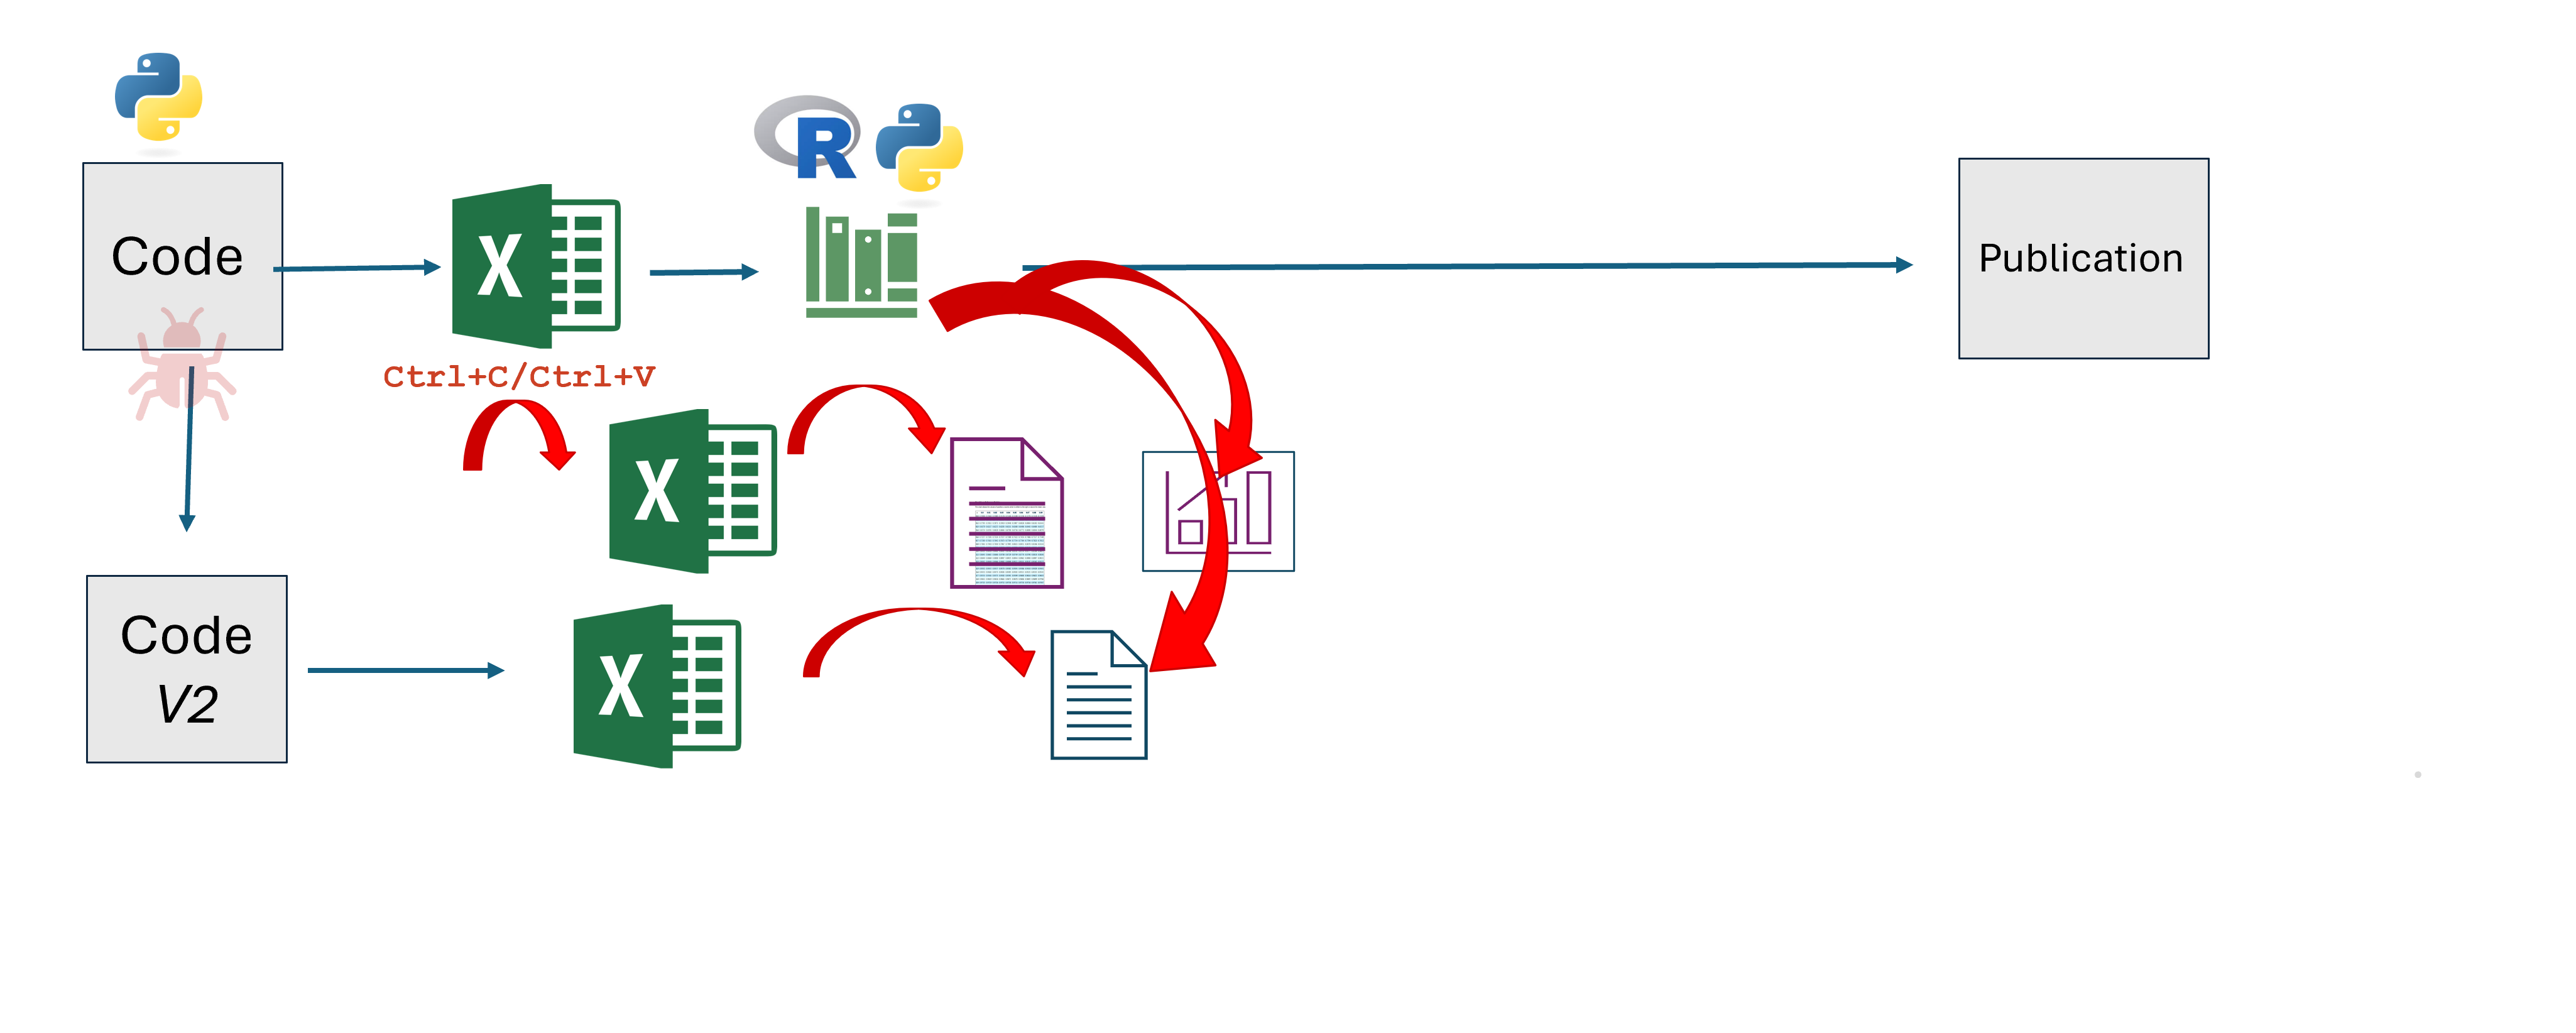
\includegraphics[width=0.8\textwidth]{Process9.png} \\ Comment 9}
        \only<10>{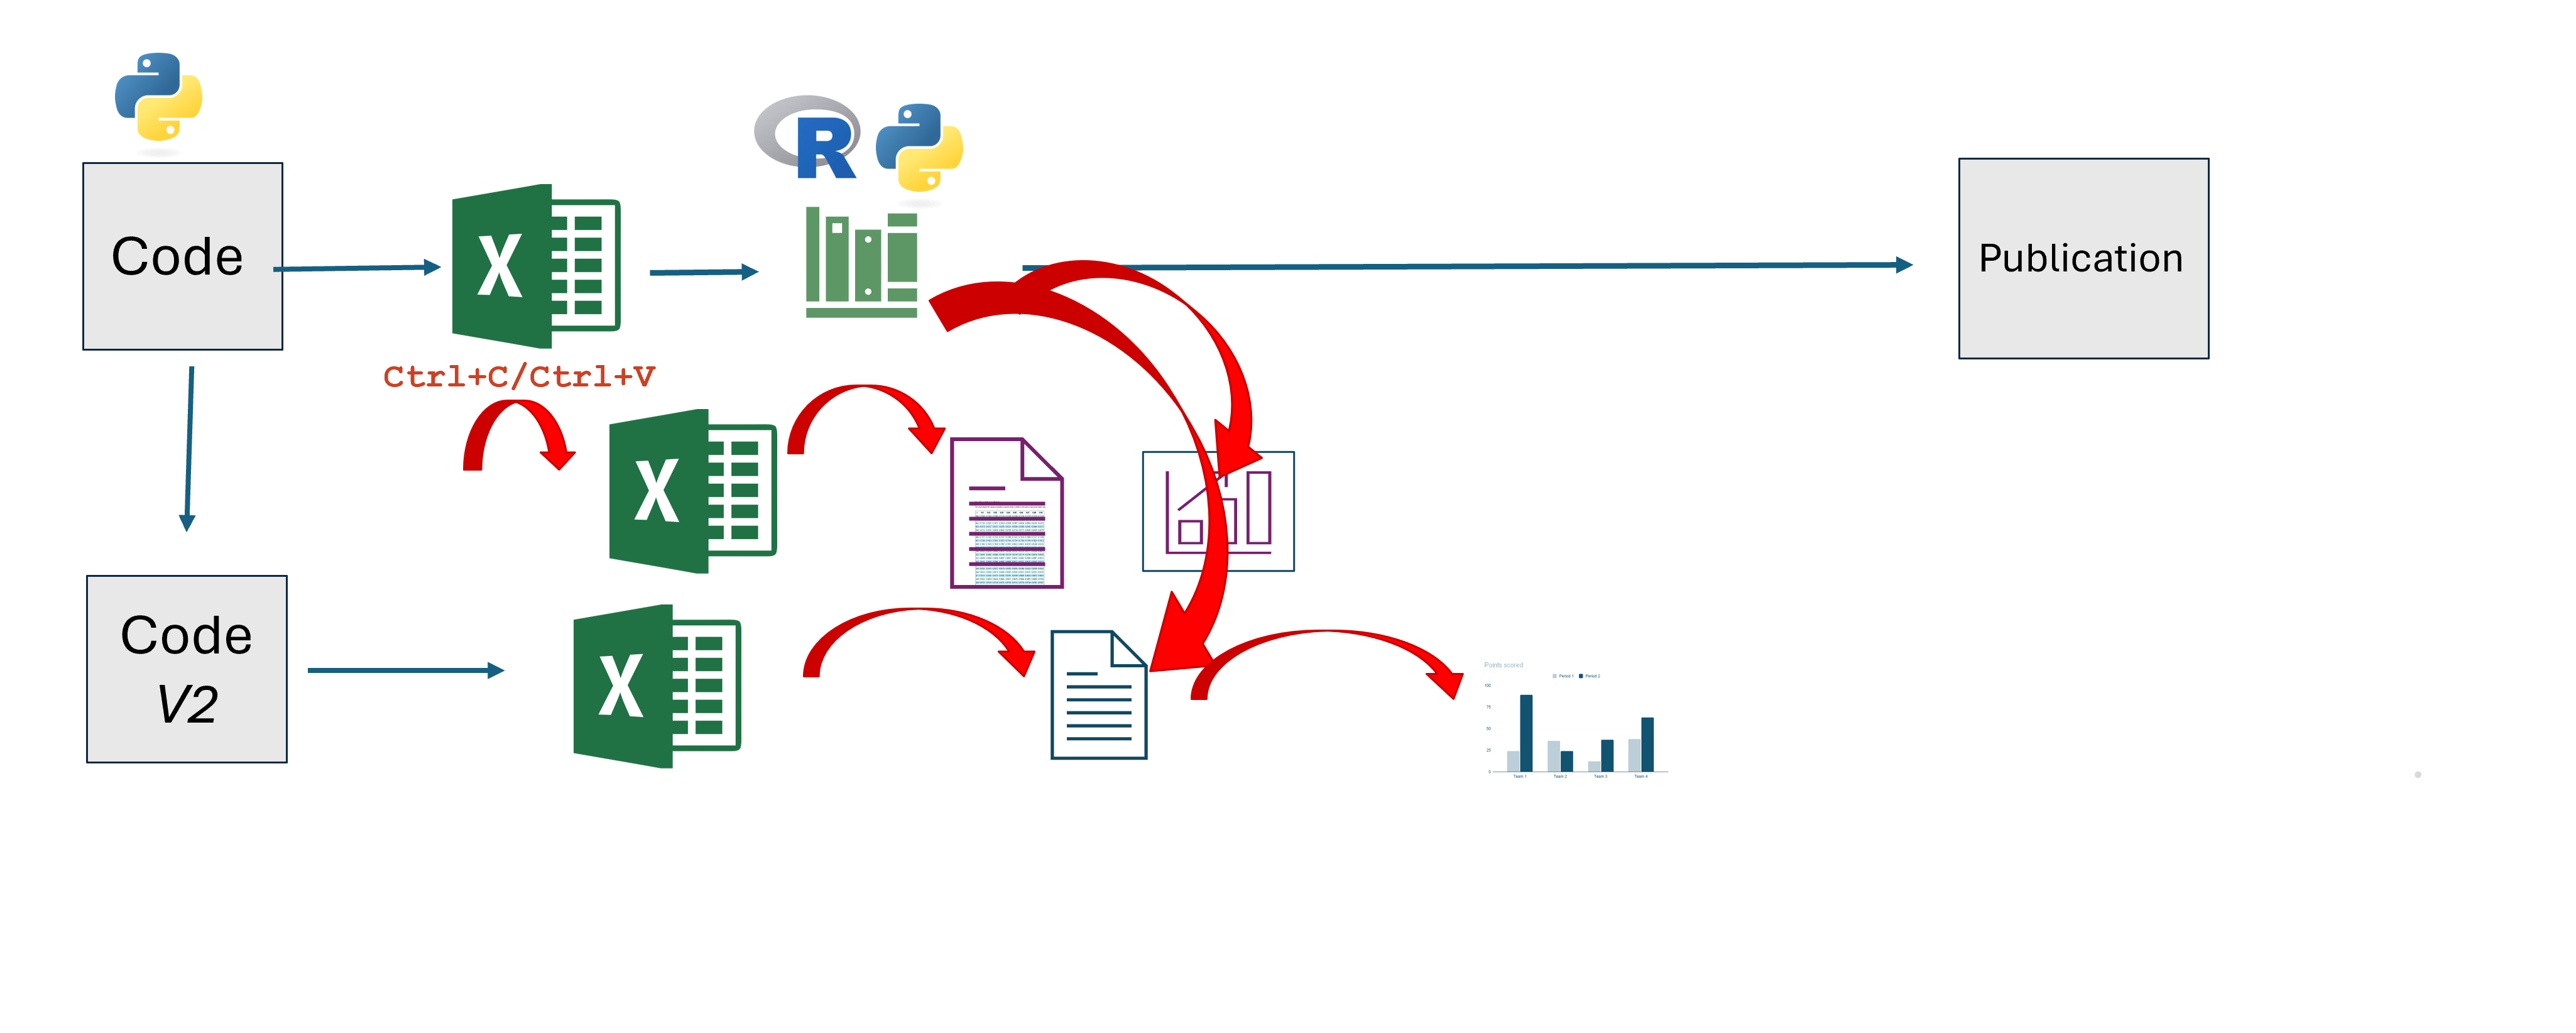
\includegraphics[width=0.8\textwidth]{Process10.png} \\ Comment 10}
        \only<11>{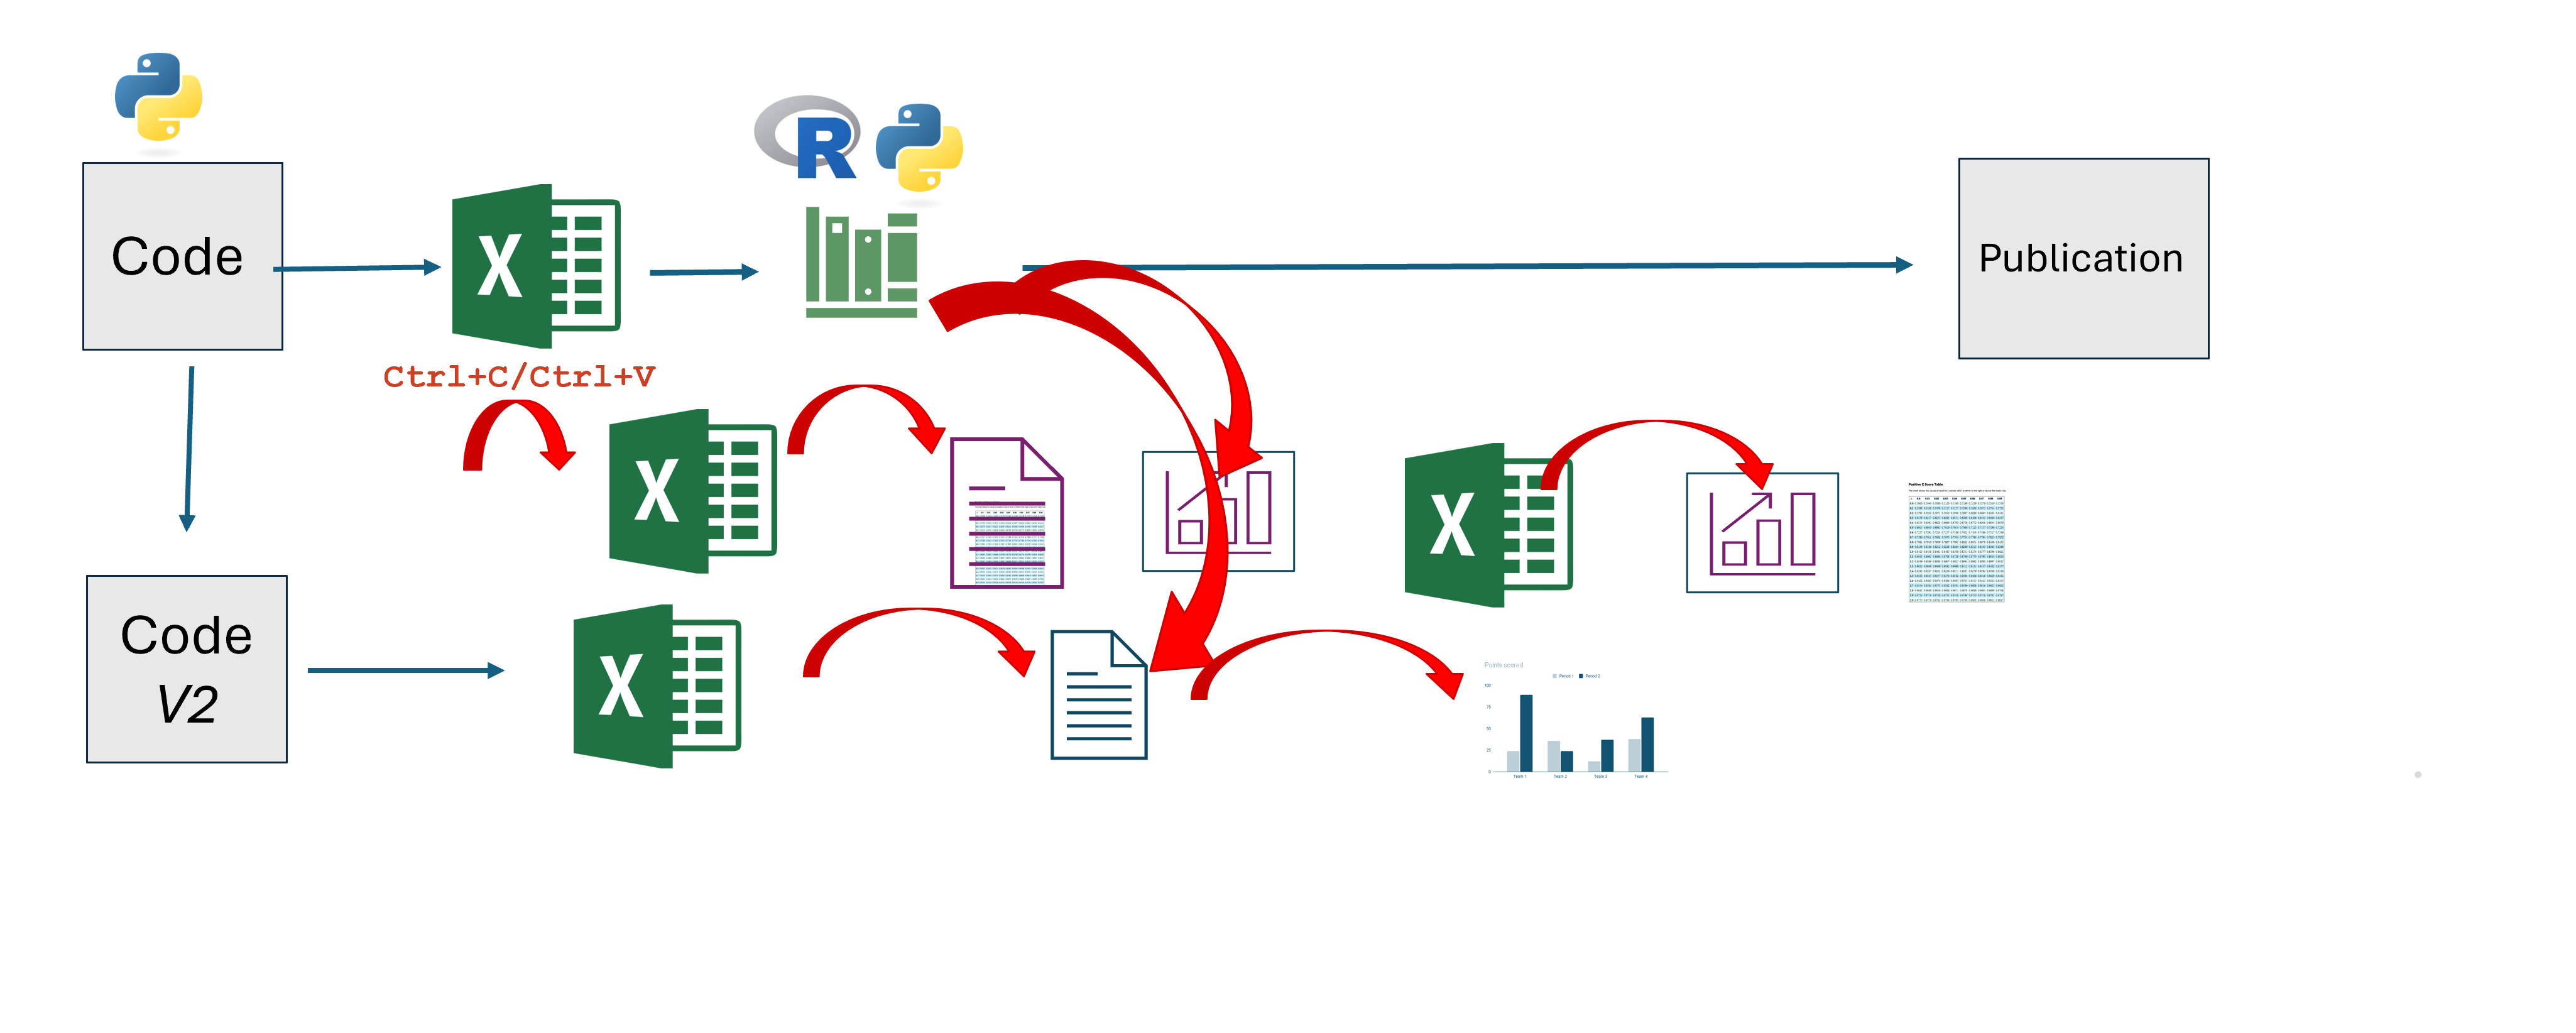
\includegraphics[width=0.8\textwidth]{Process11.png} \\ Comment 9}
        \only<12>{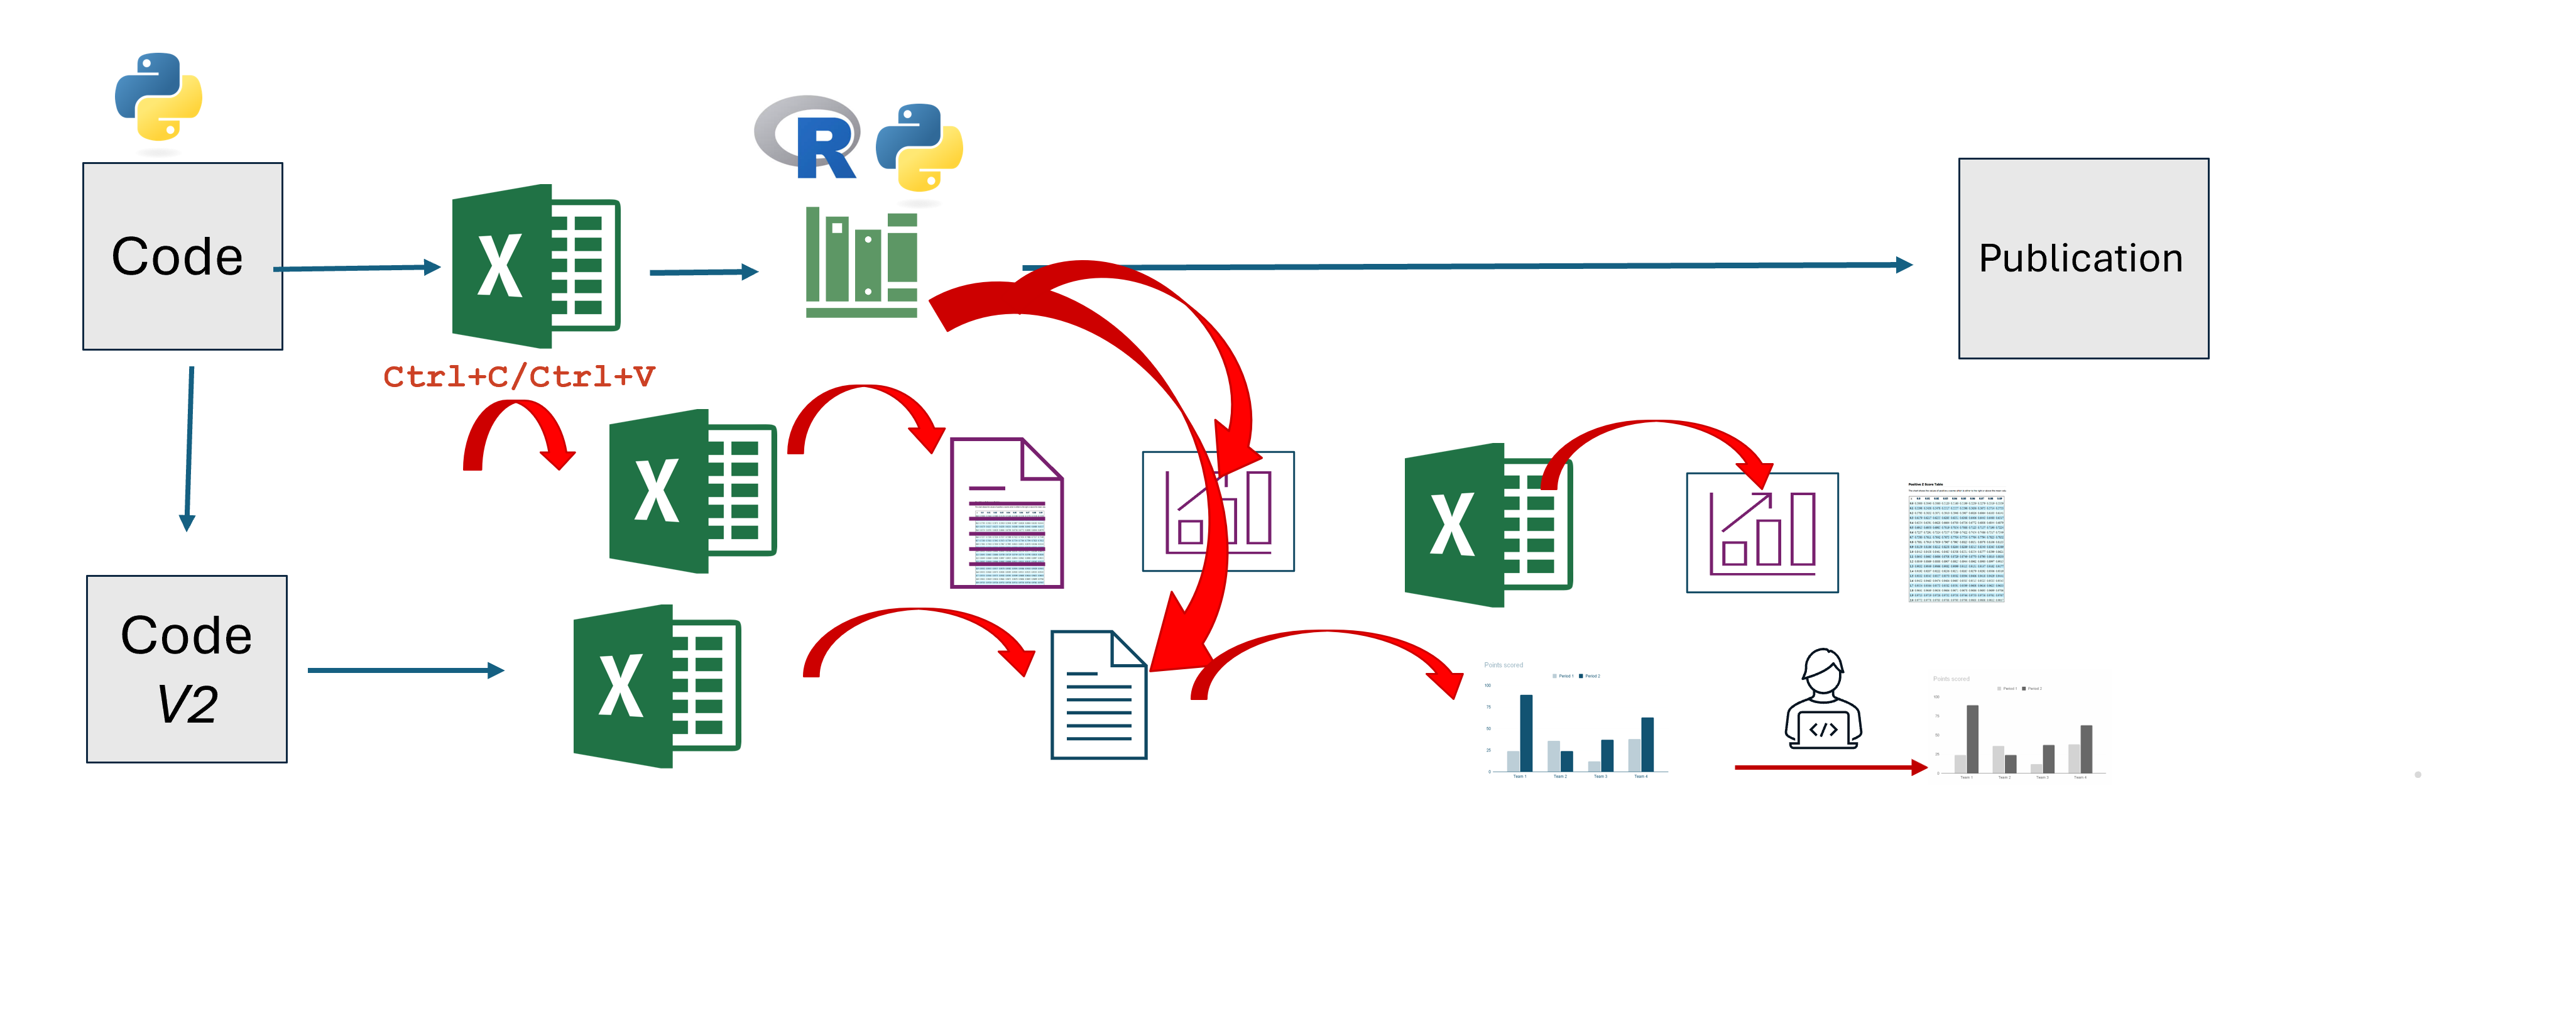
\includegraphics[width=0.8\textwidth]{Process12.png} \\ Comment 10}  
        \only<13>{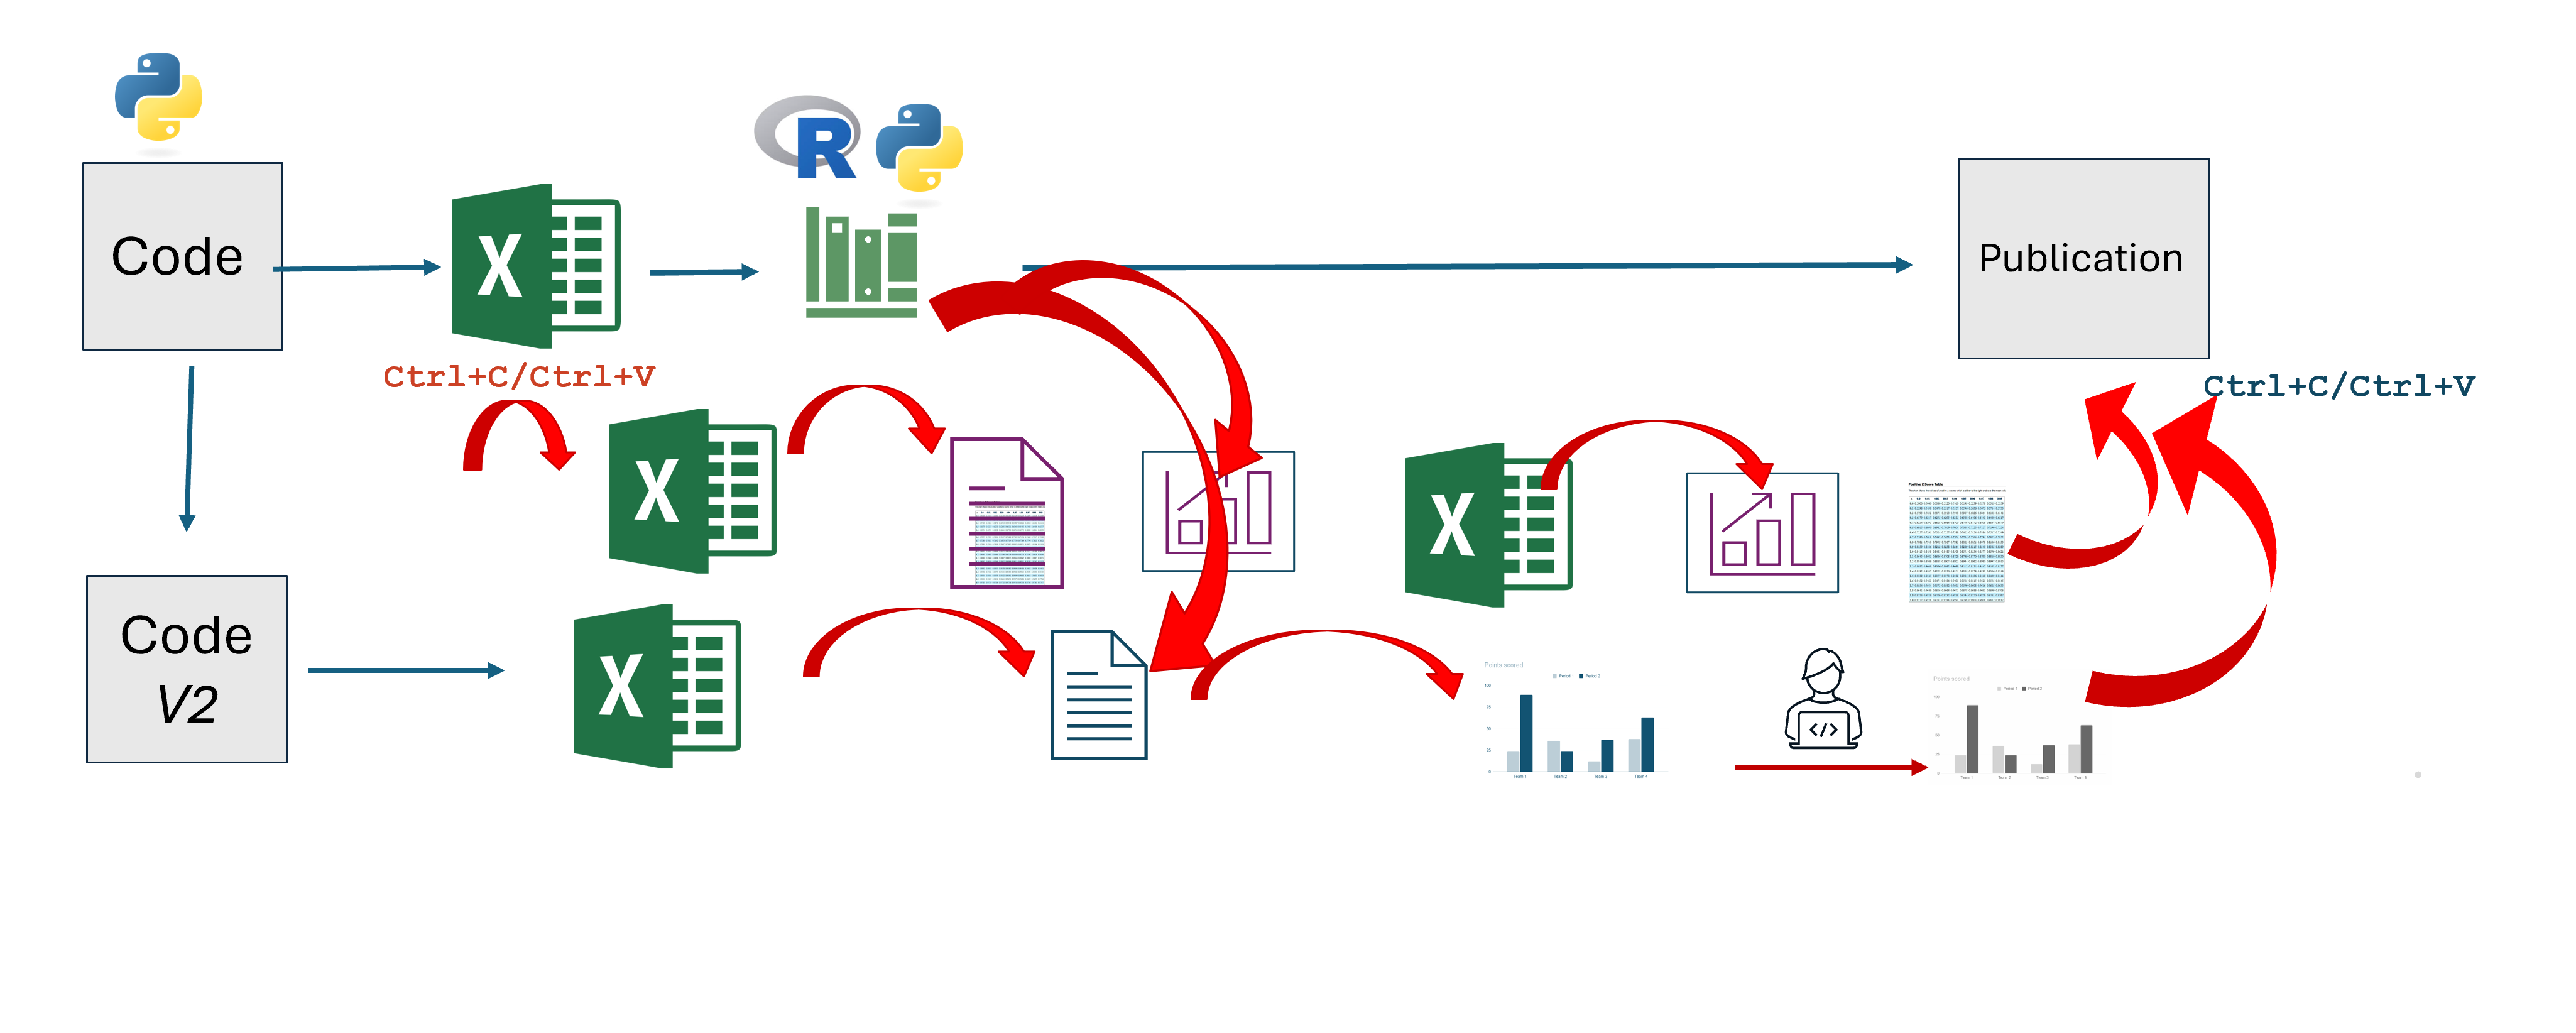
\includegraphics[width=0.8\textwidth]{Process13.png} \\ Comment 9}
        \only<14>{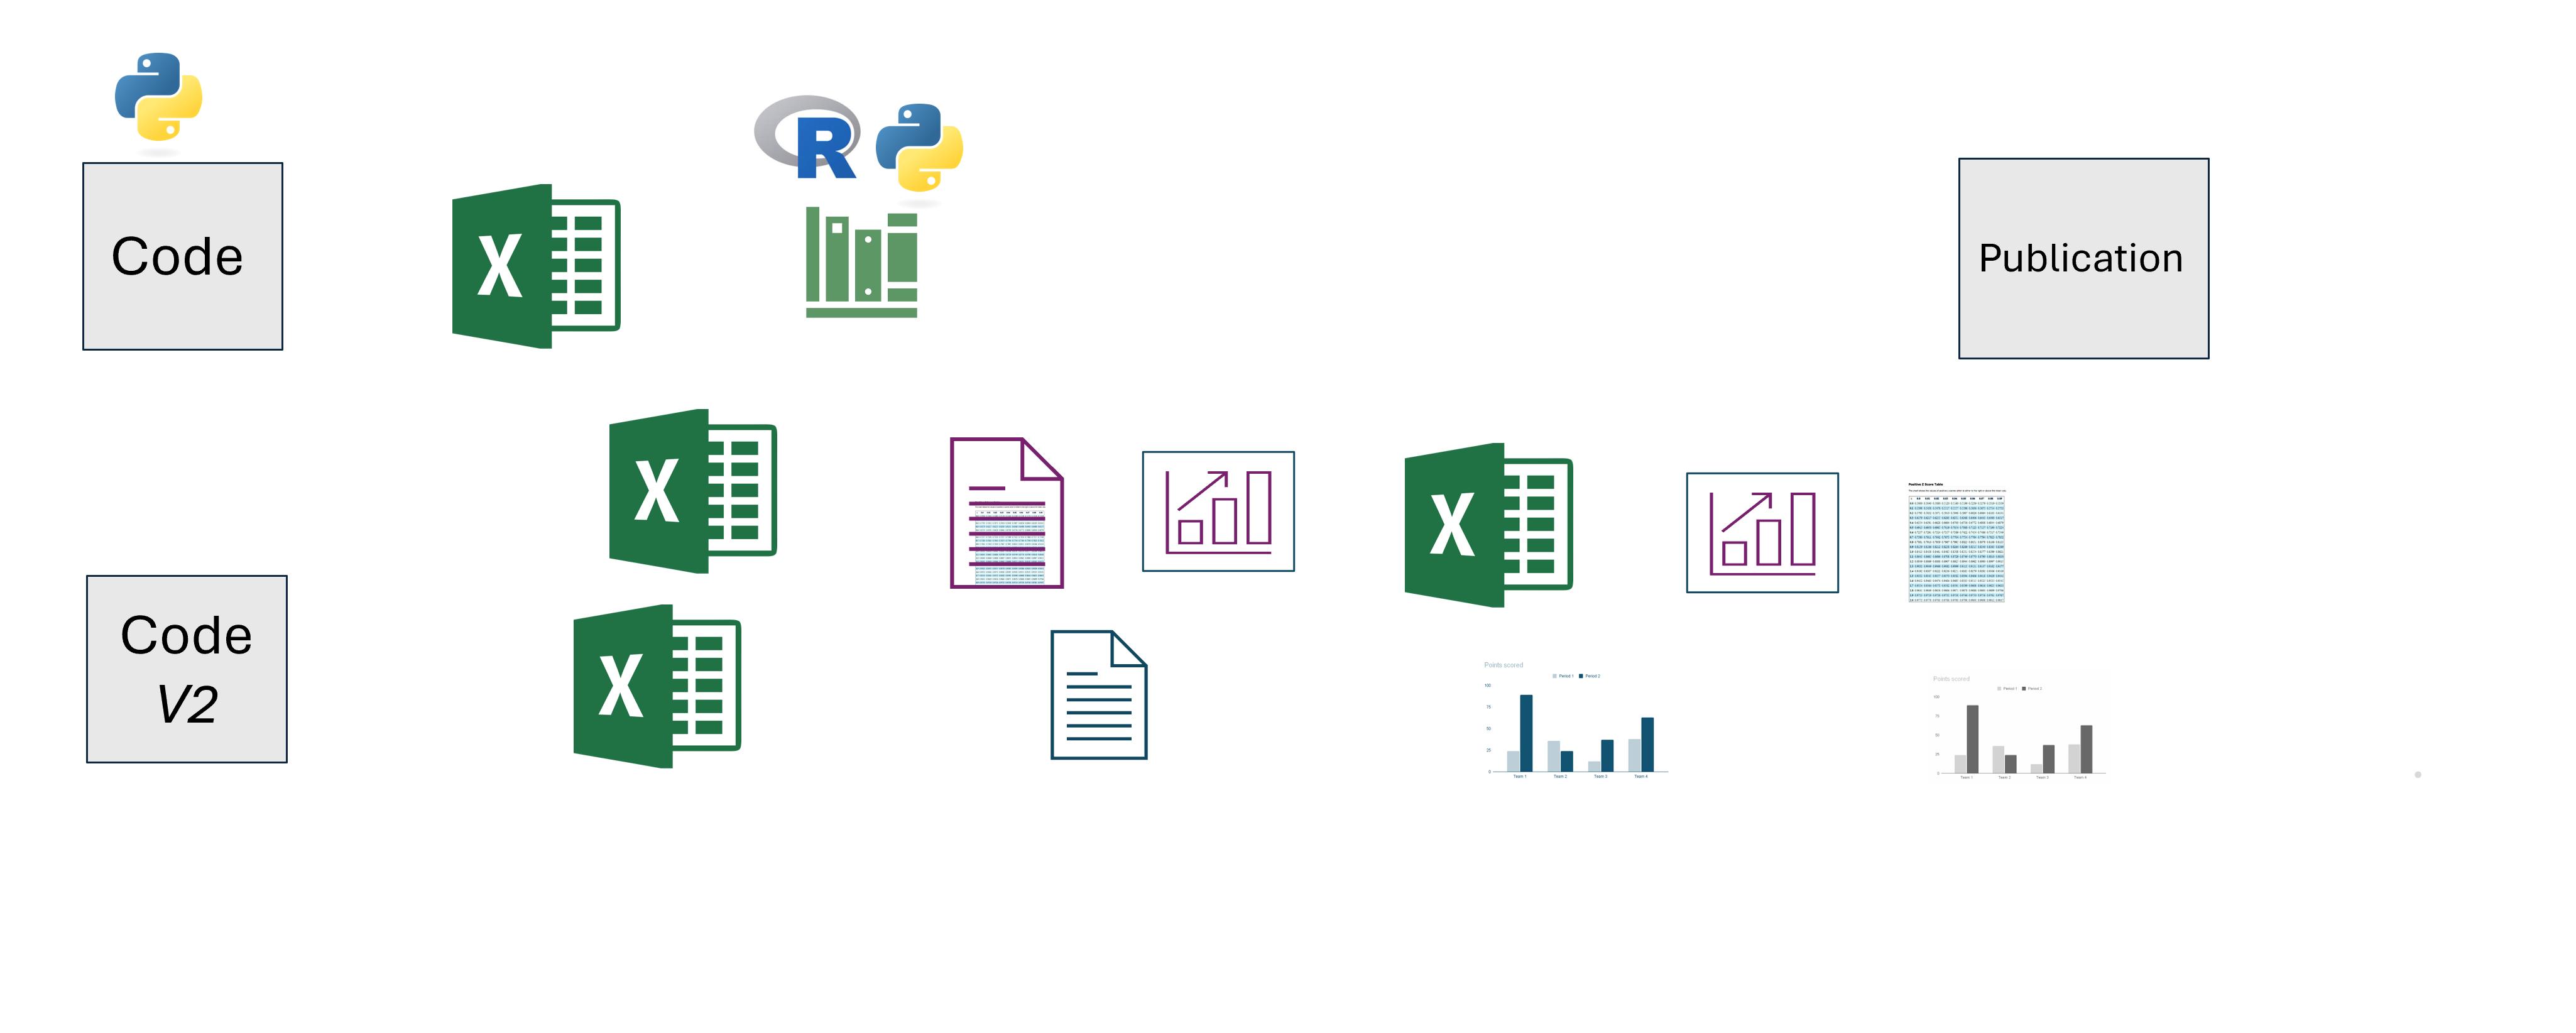
\includegraphics[width=0.8\textwidth]{Process14.png} \\ Comment 10}         
    \end{itemize}
\end{center}
\end{frame}


\begin{frame}{Usual practice: In the end}

 \begin{columns}[T]
    \begin{column}{0.5\textwidth}
      \begin{itemize}[<+->]
        \item Lots of files
        \item Cut and paste is not a reliable, reproducible approach!
        \item Your brain may remember..
        \item[] ...all the steps...
        \item[] .. in the right order..
        \item[]...all of them !
        \item Or use (bad) "\emph{tools}" 
      \end{itemize}
    \end{column}
    \begin{column}{0.5\textwidth}
       \begin{itemize}
       \item[] \only<1>{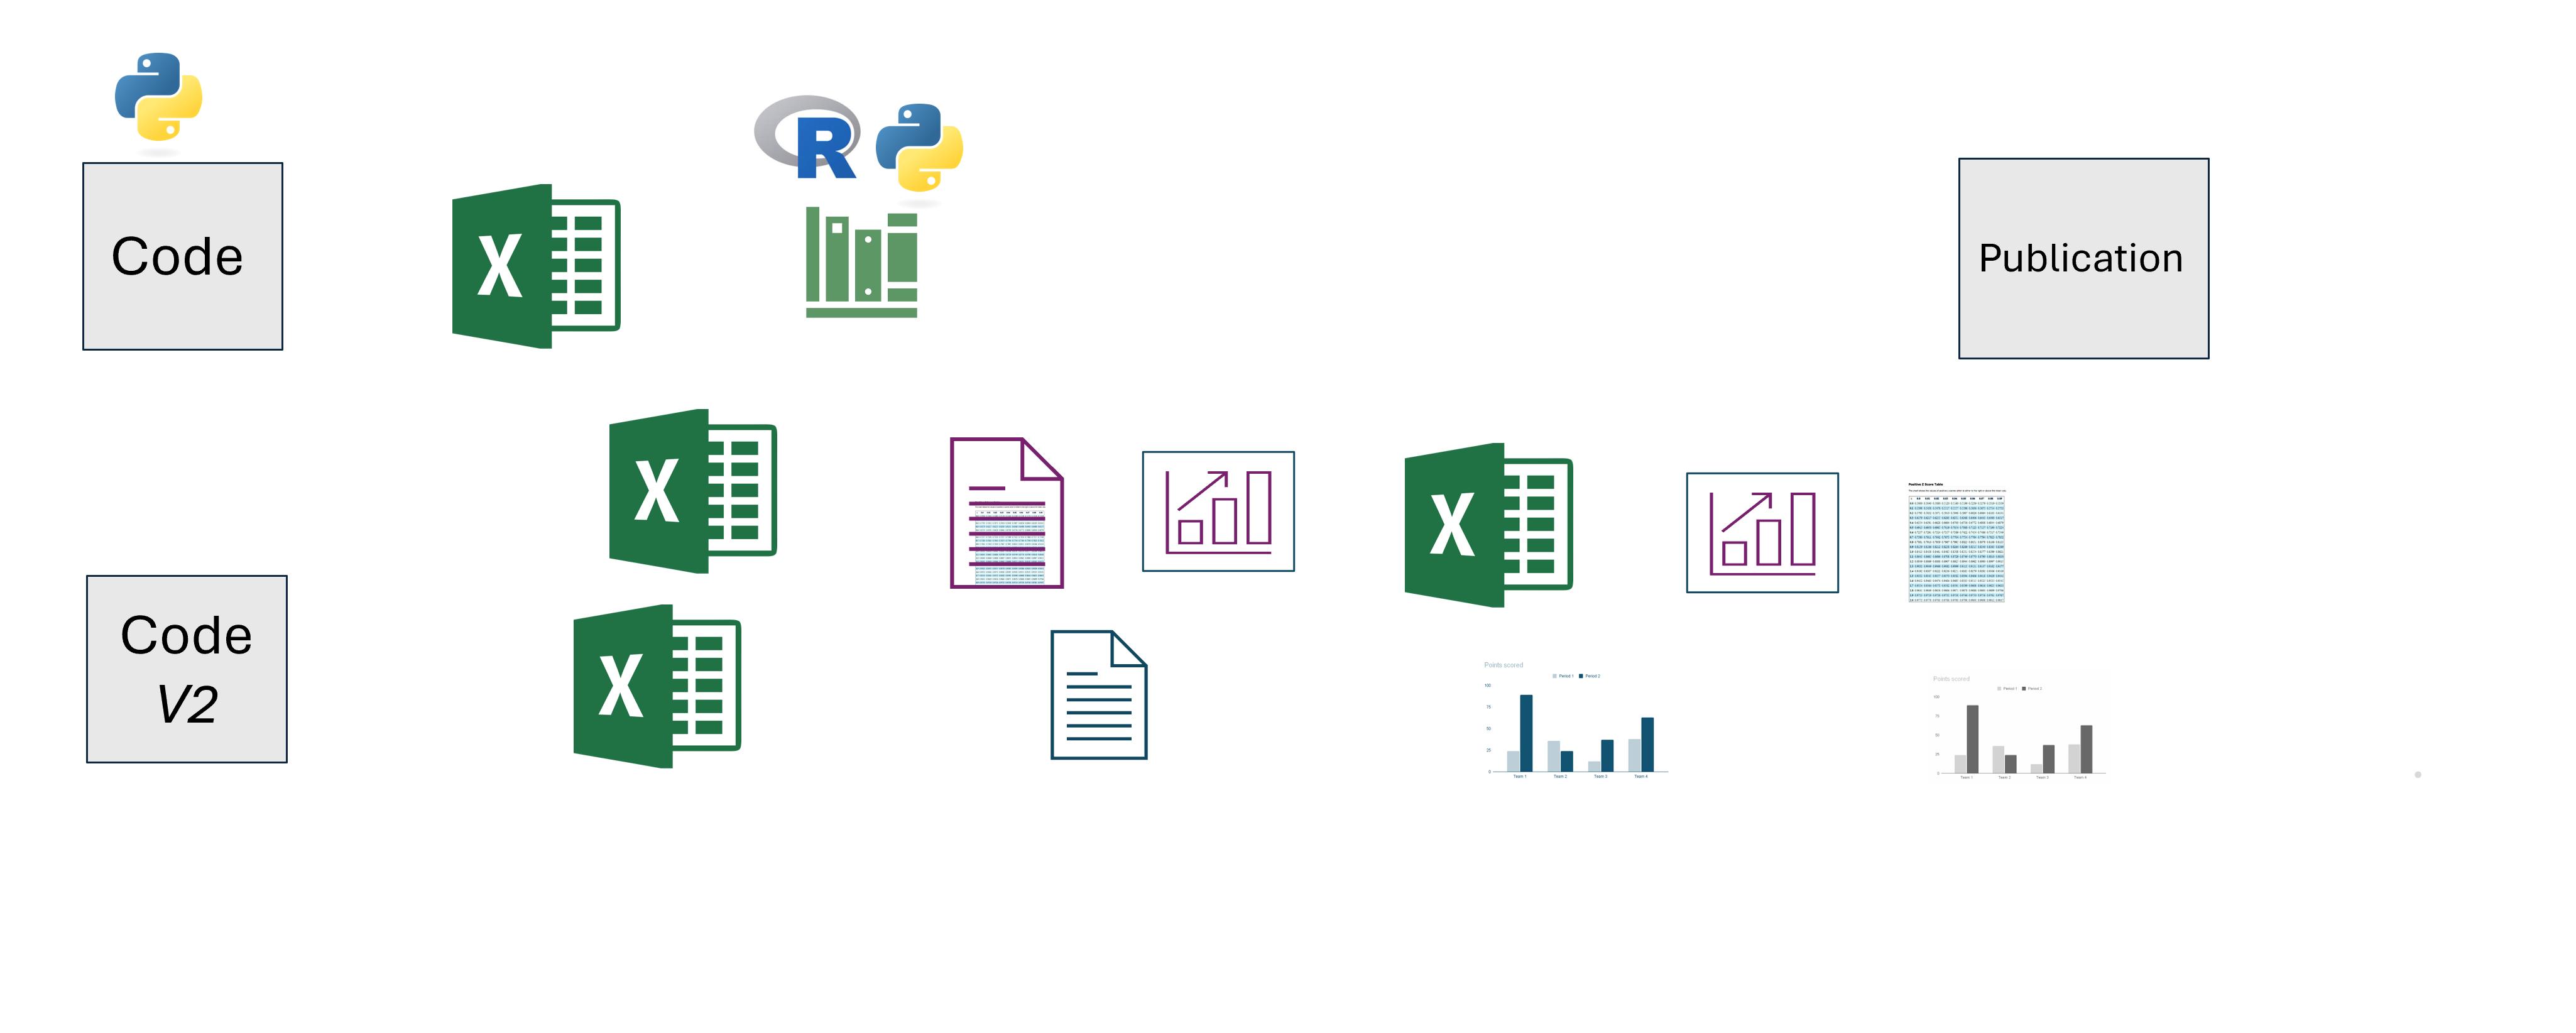
\includegraphics[width=0.8\textwidth]{Process14.png} }
        \only<2>{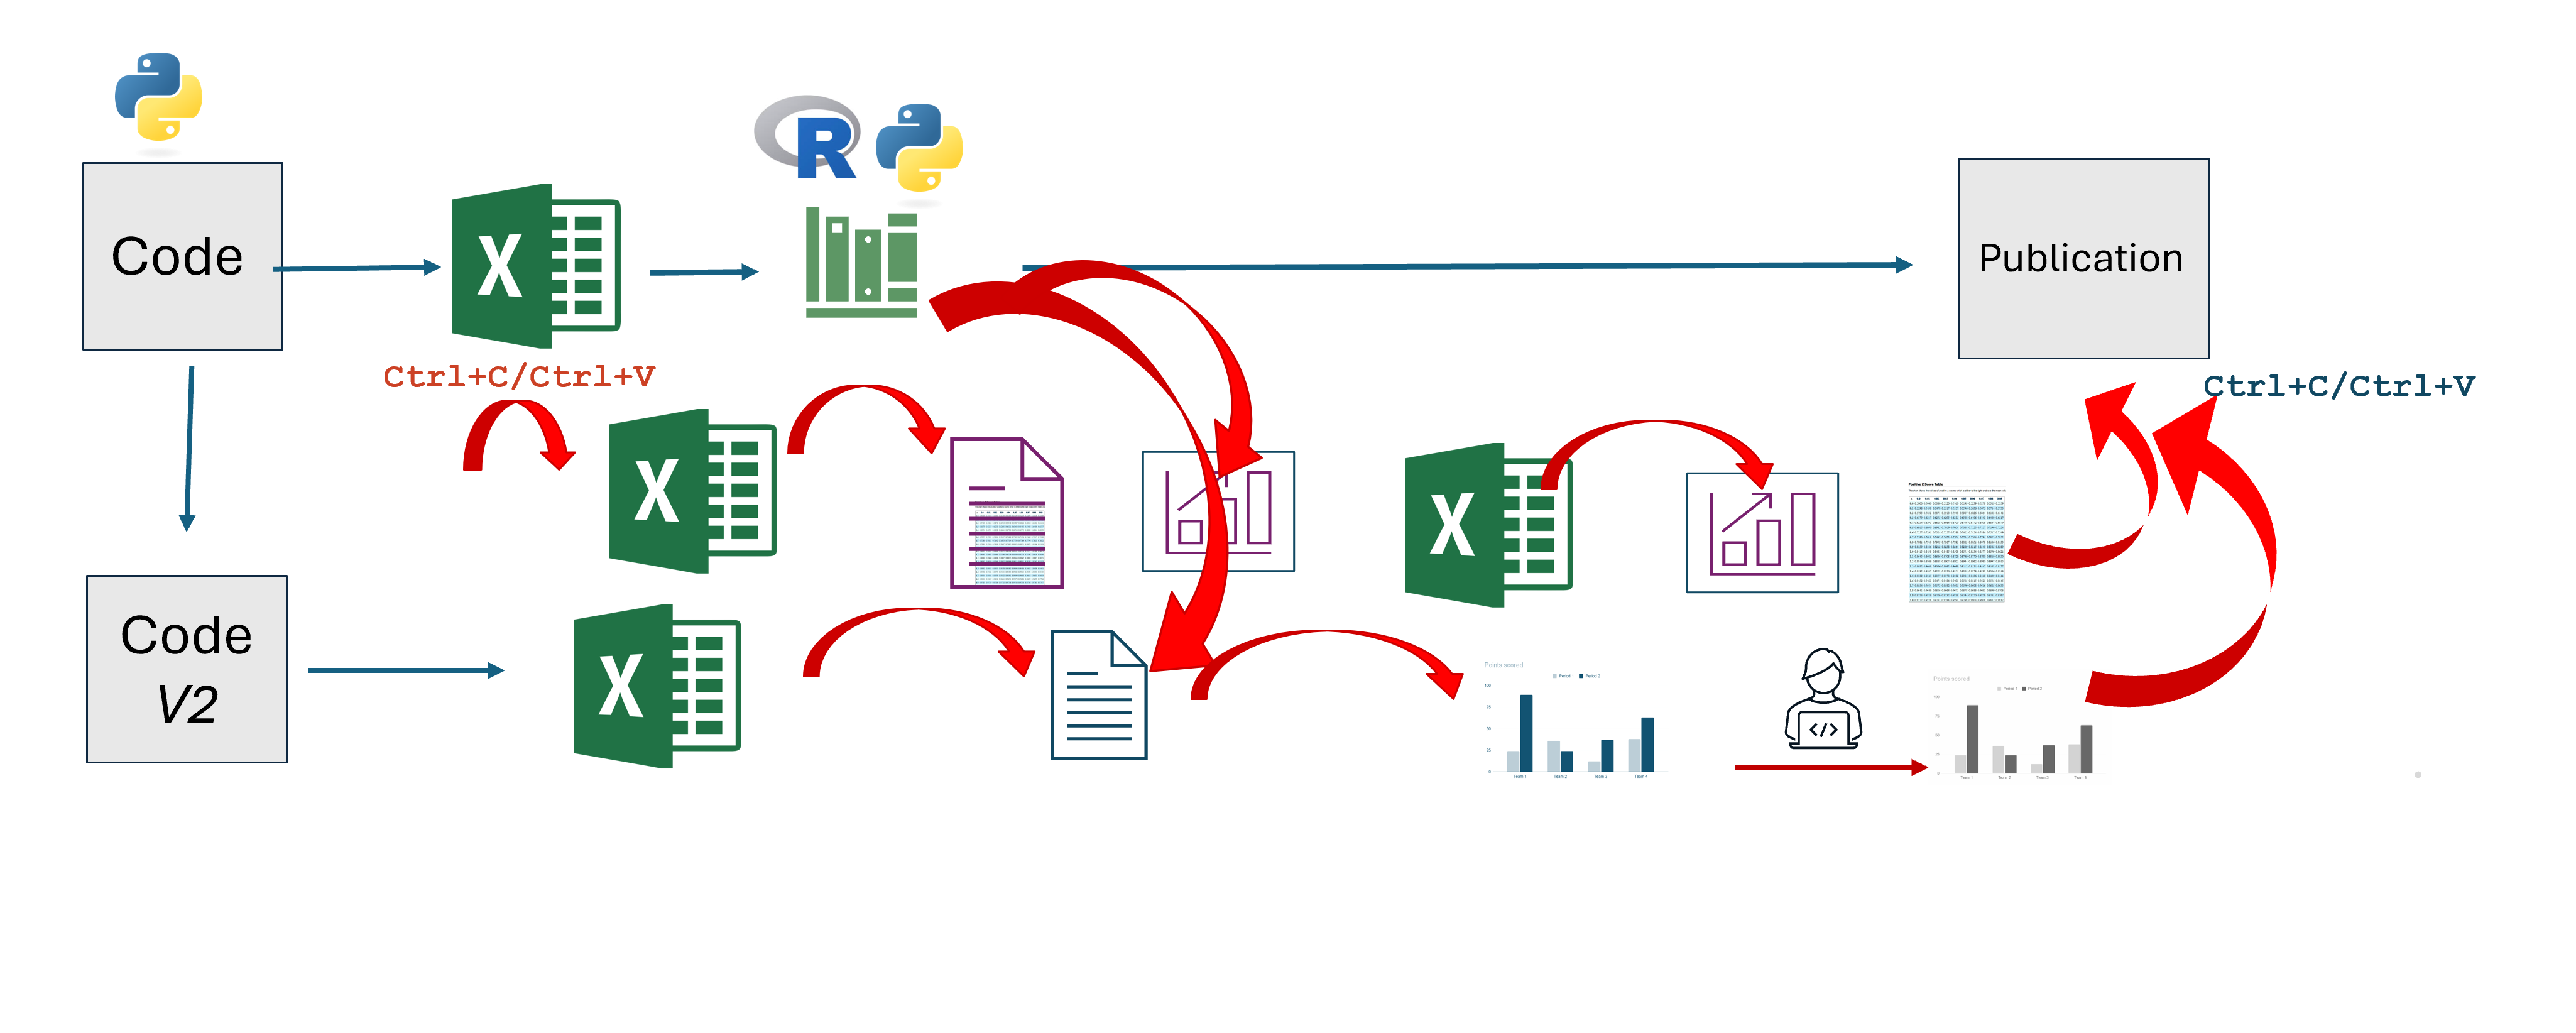
\includegraphics[width=1.0\textwidth]{Process13.png} }
        \only<3>{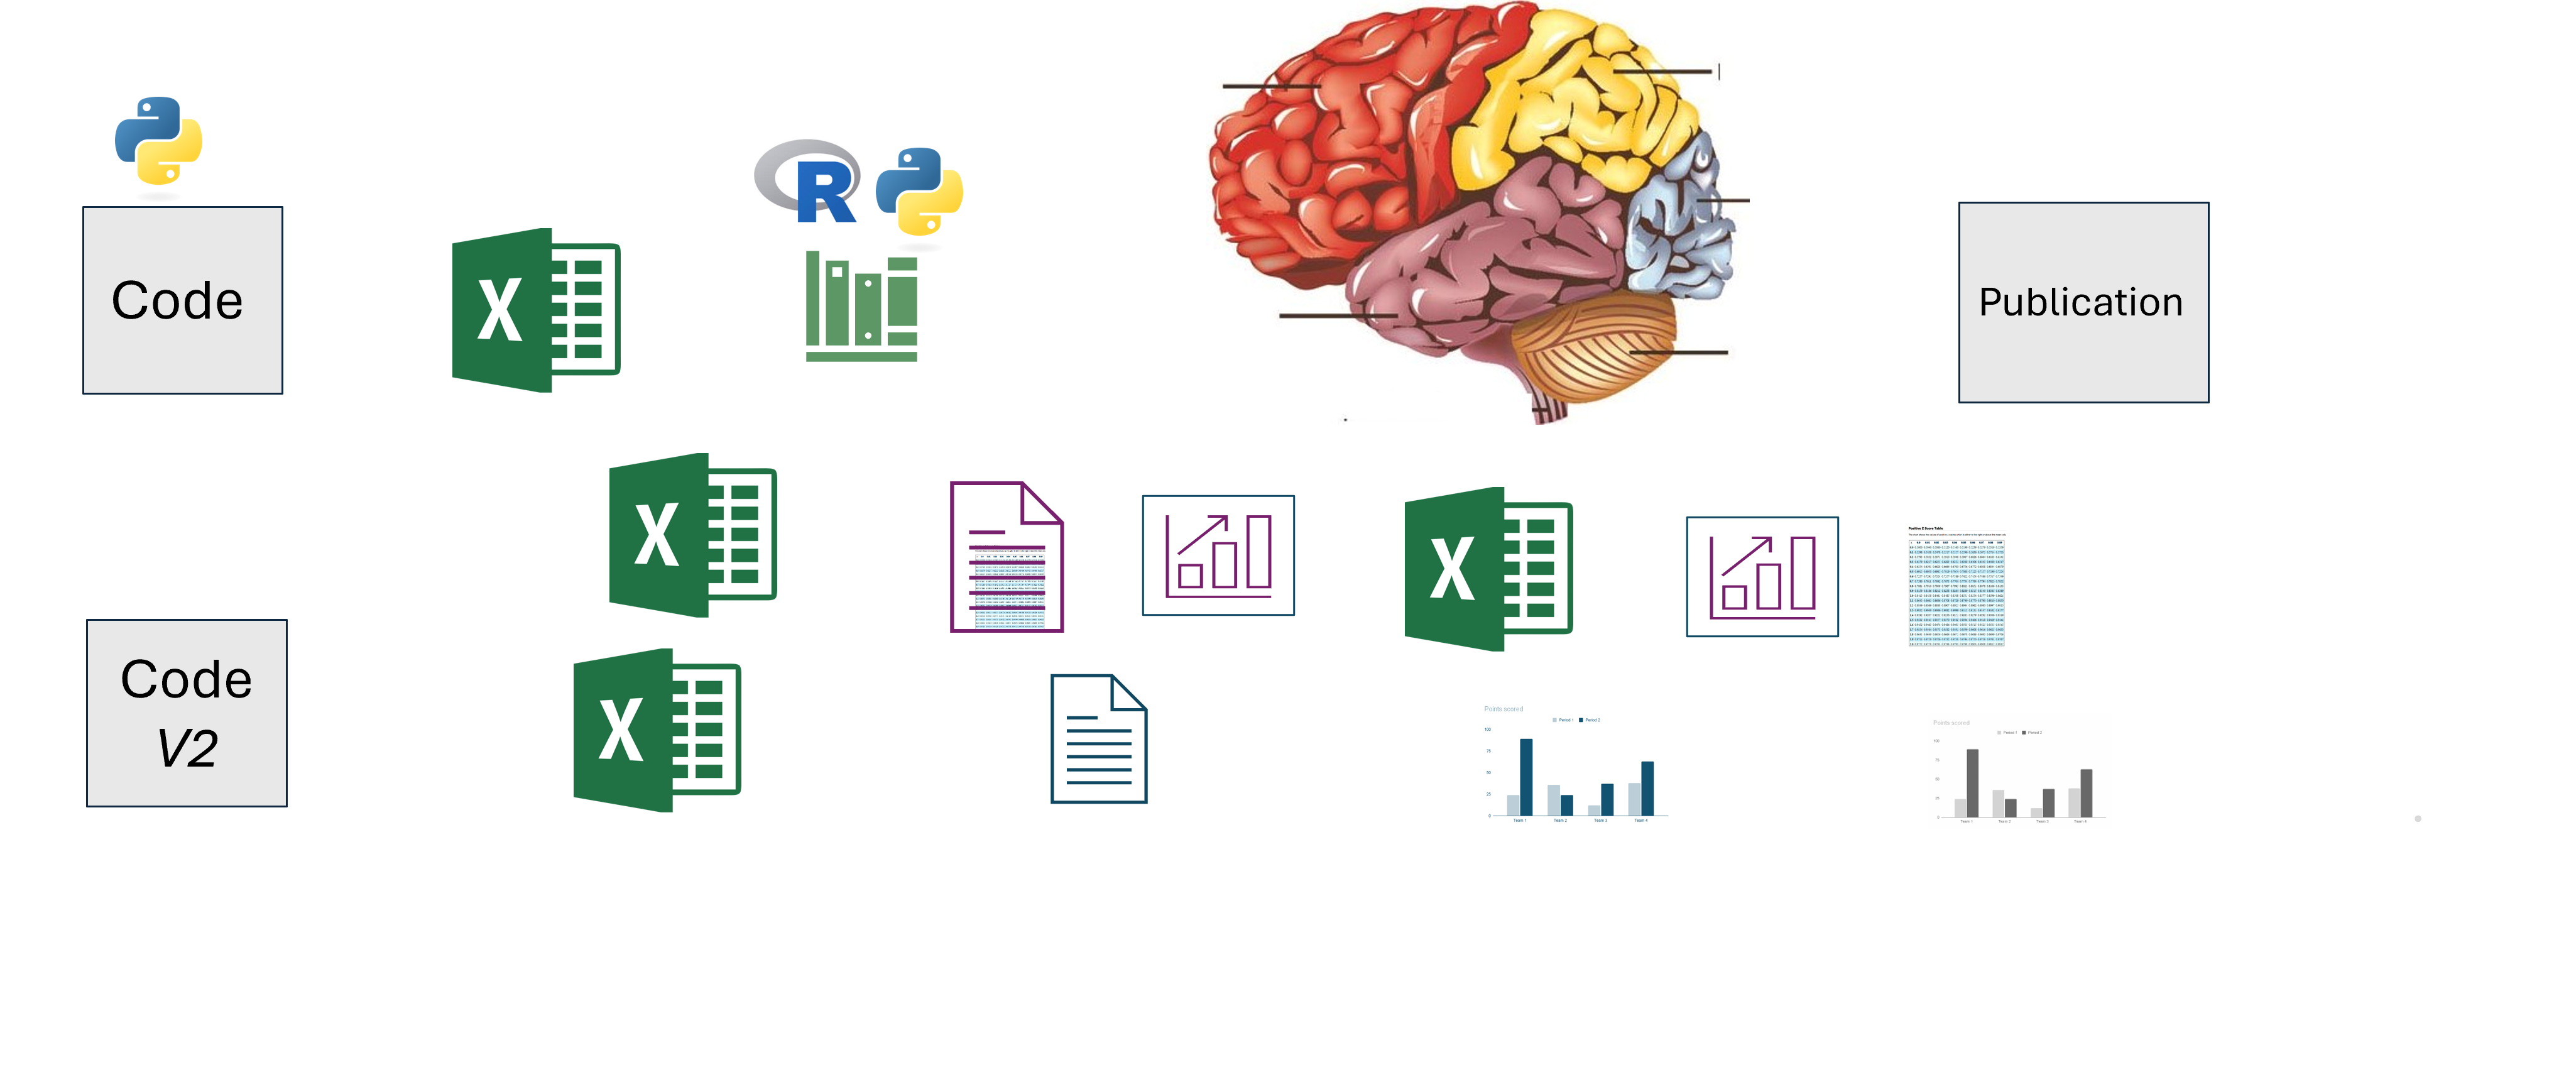
\includegraphics[width=1.0\textwidth]{Process15.png} }
        \only<4>{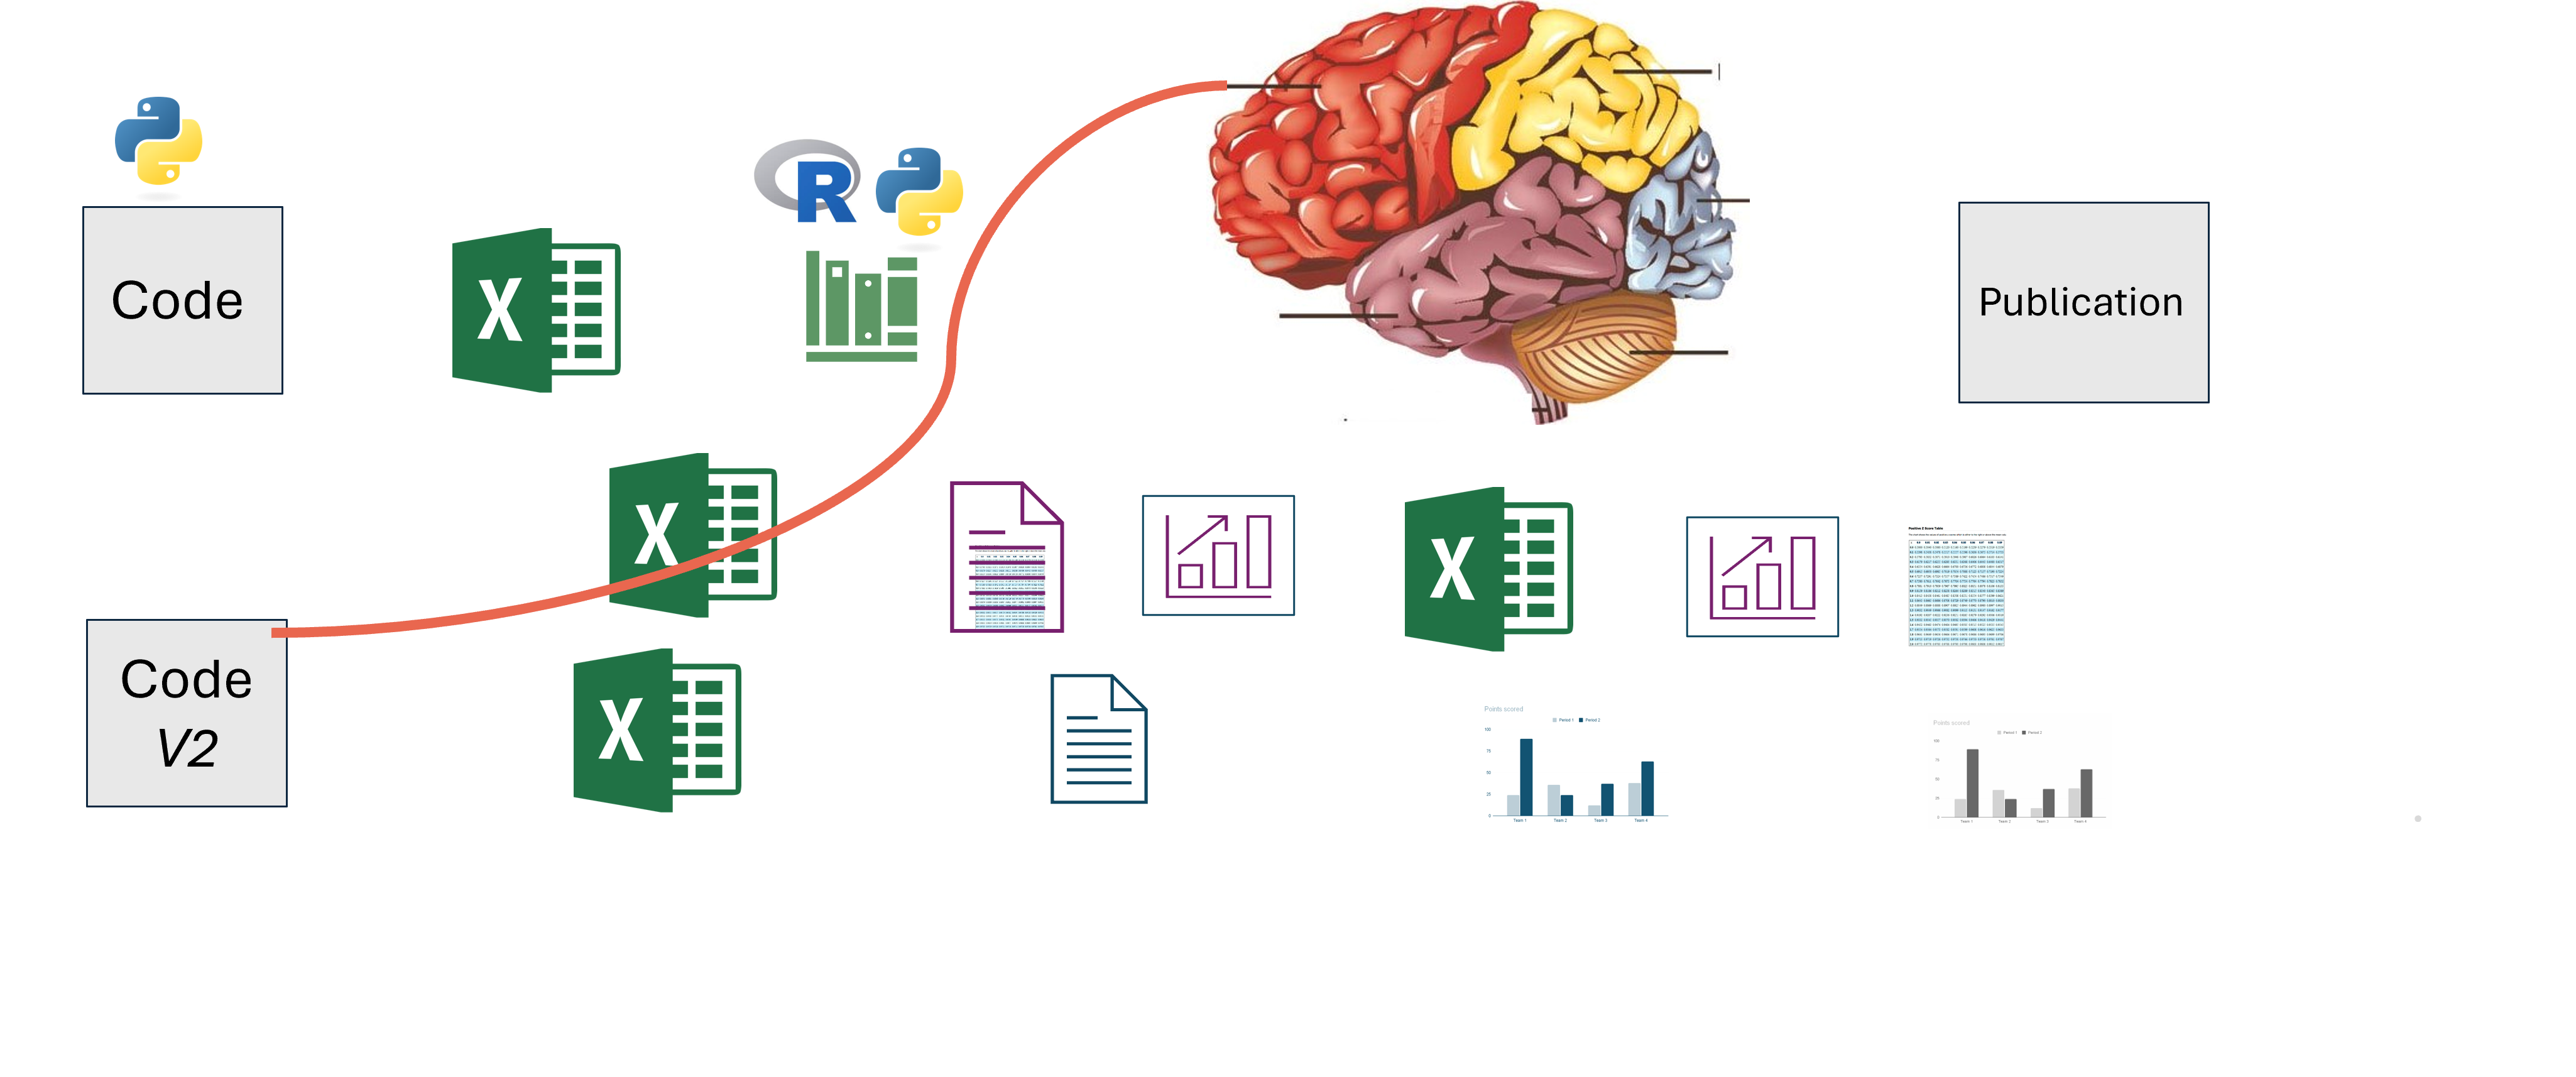
\includegraphics[width=1.0\textwidth]{Process16.png} }
        \only<5>{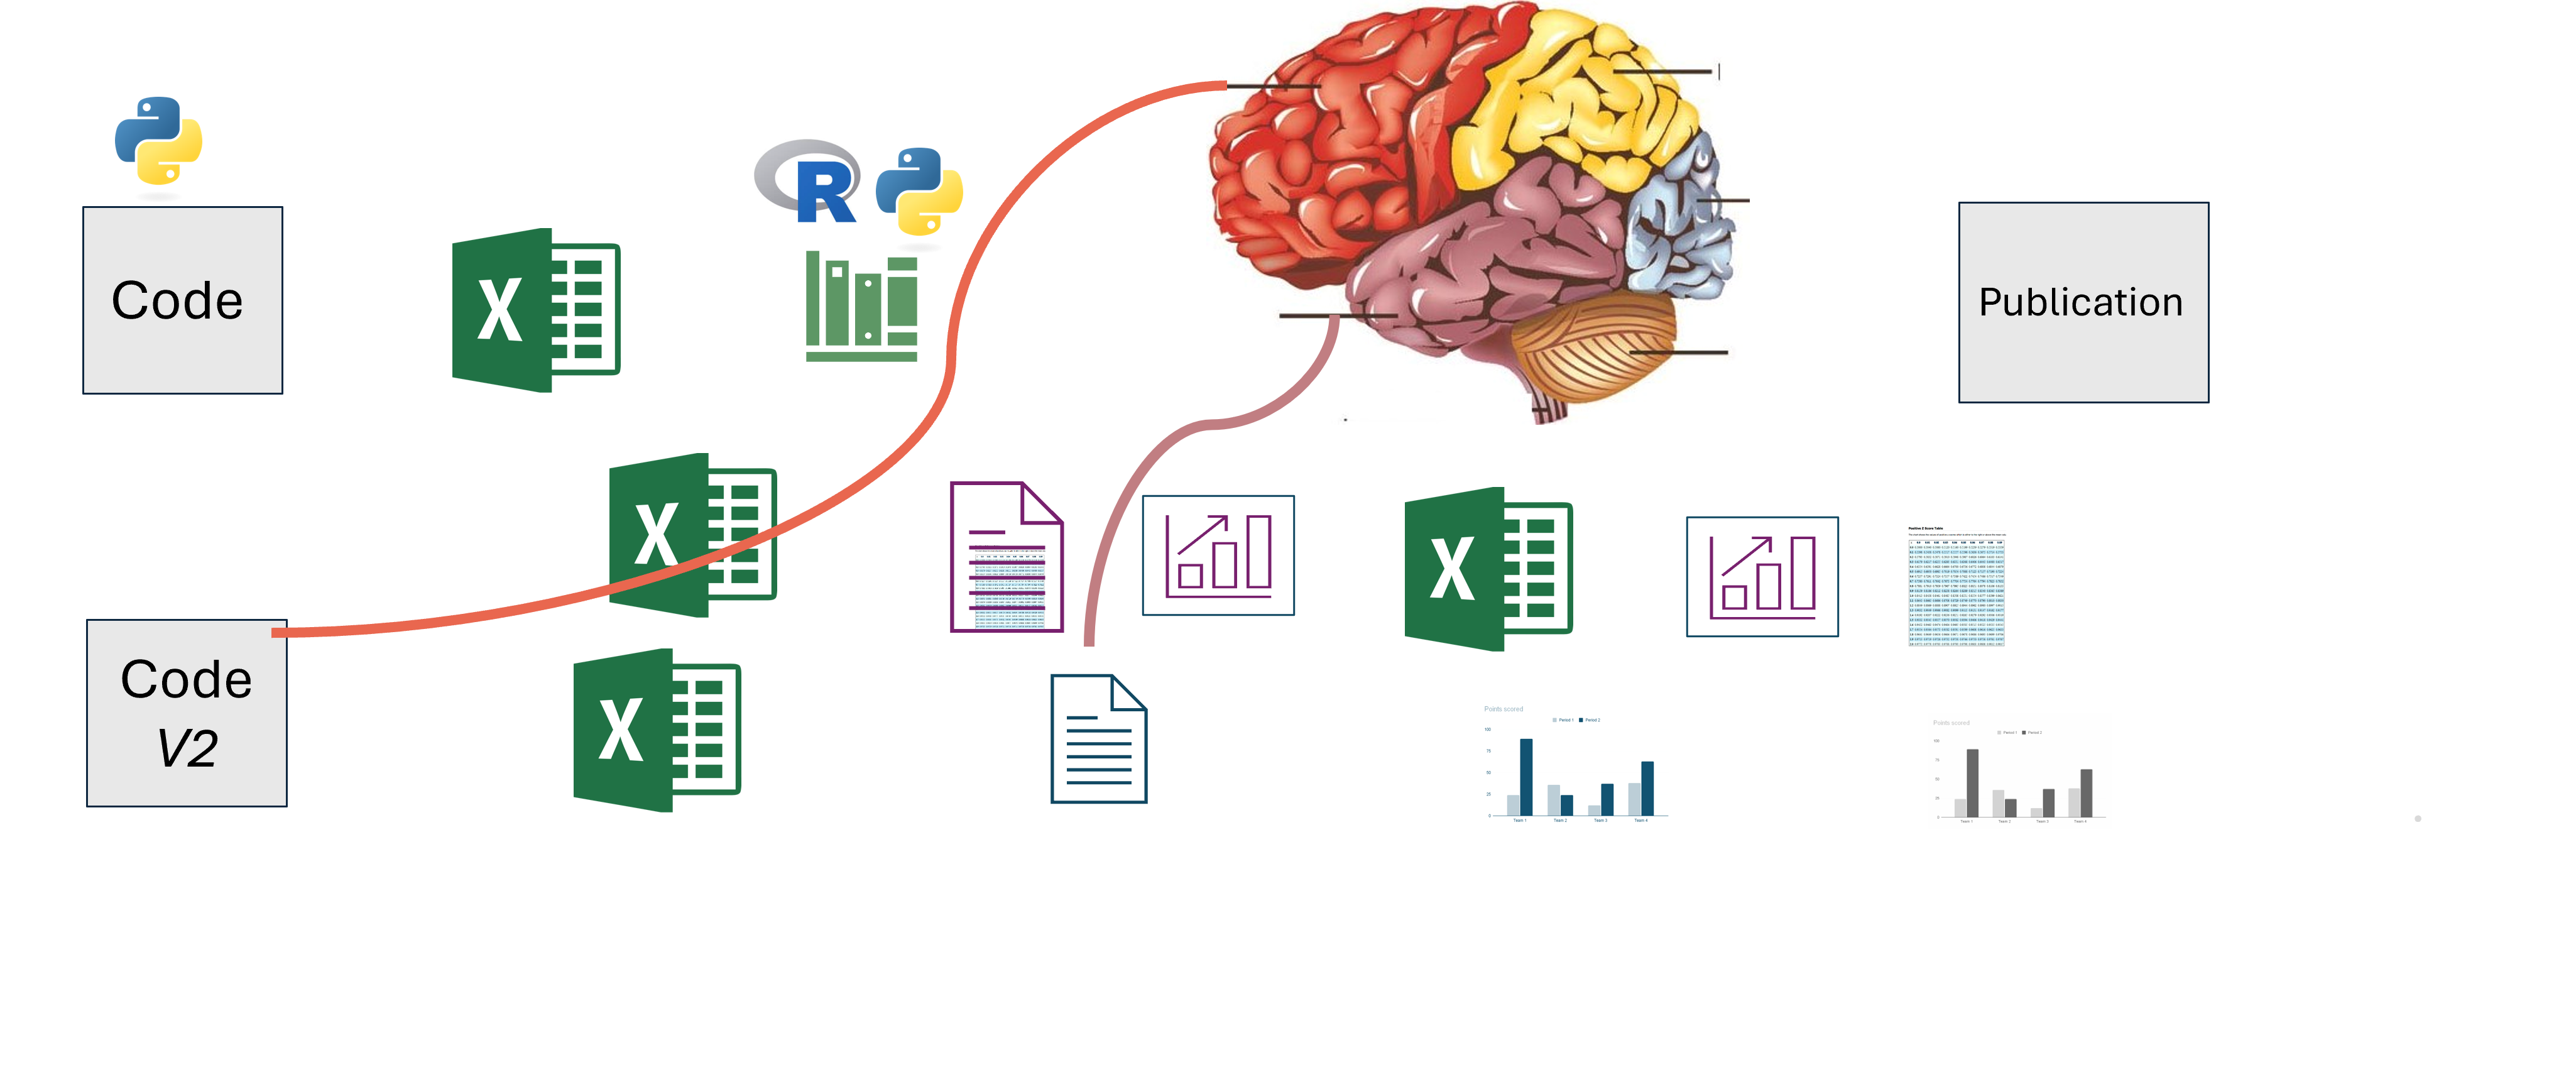
\includegraphics[width=1.0\textwidth]{Process17.png}}
        \only<6>{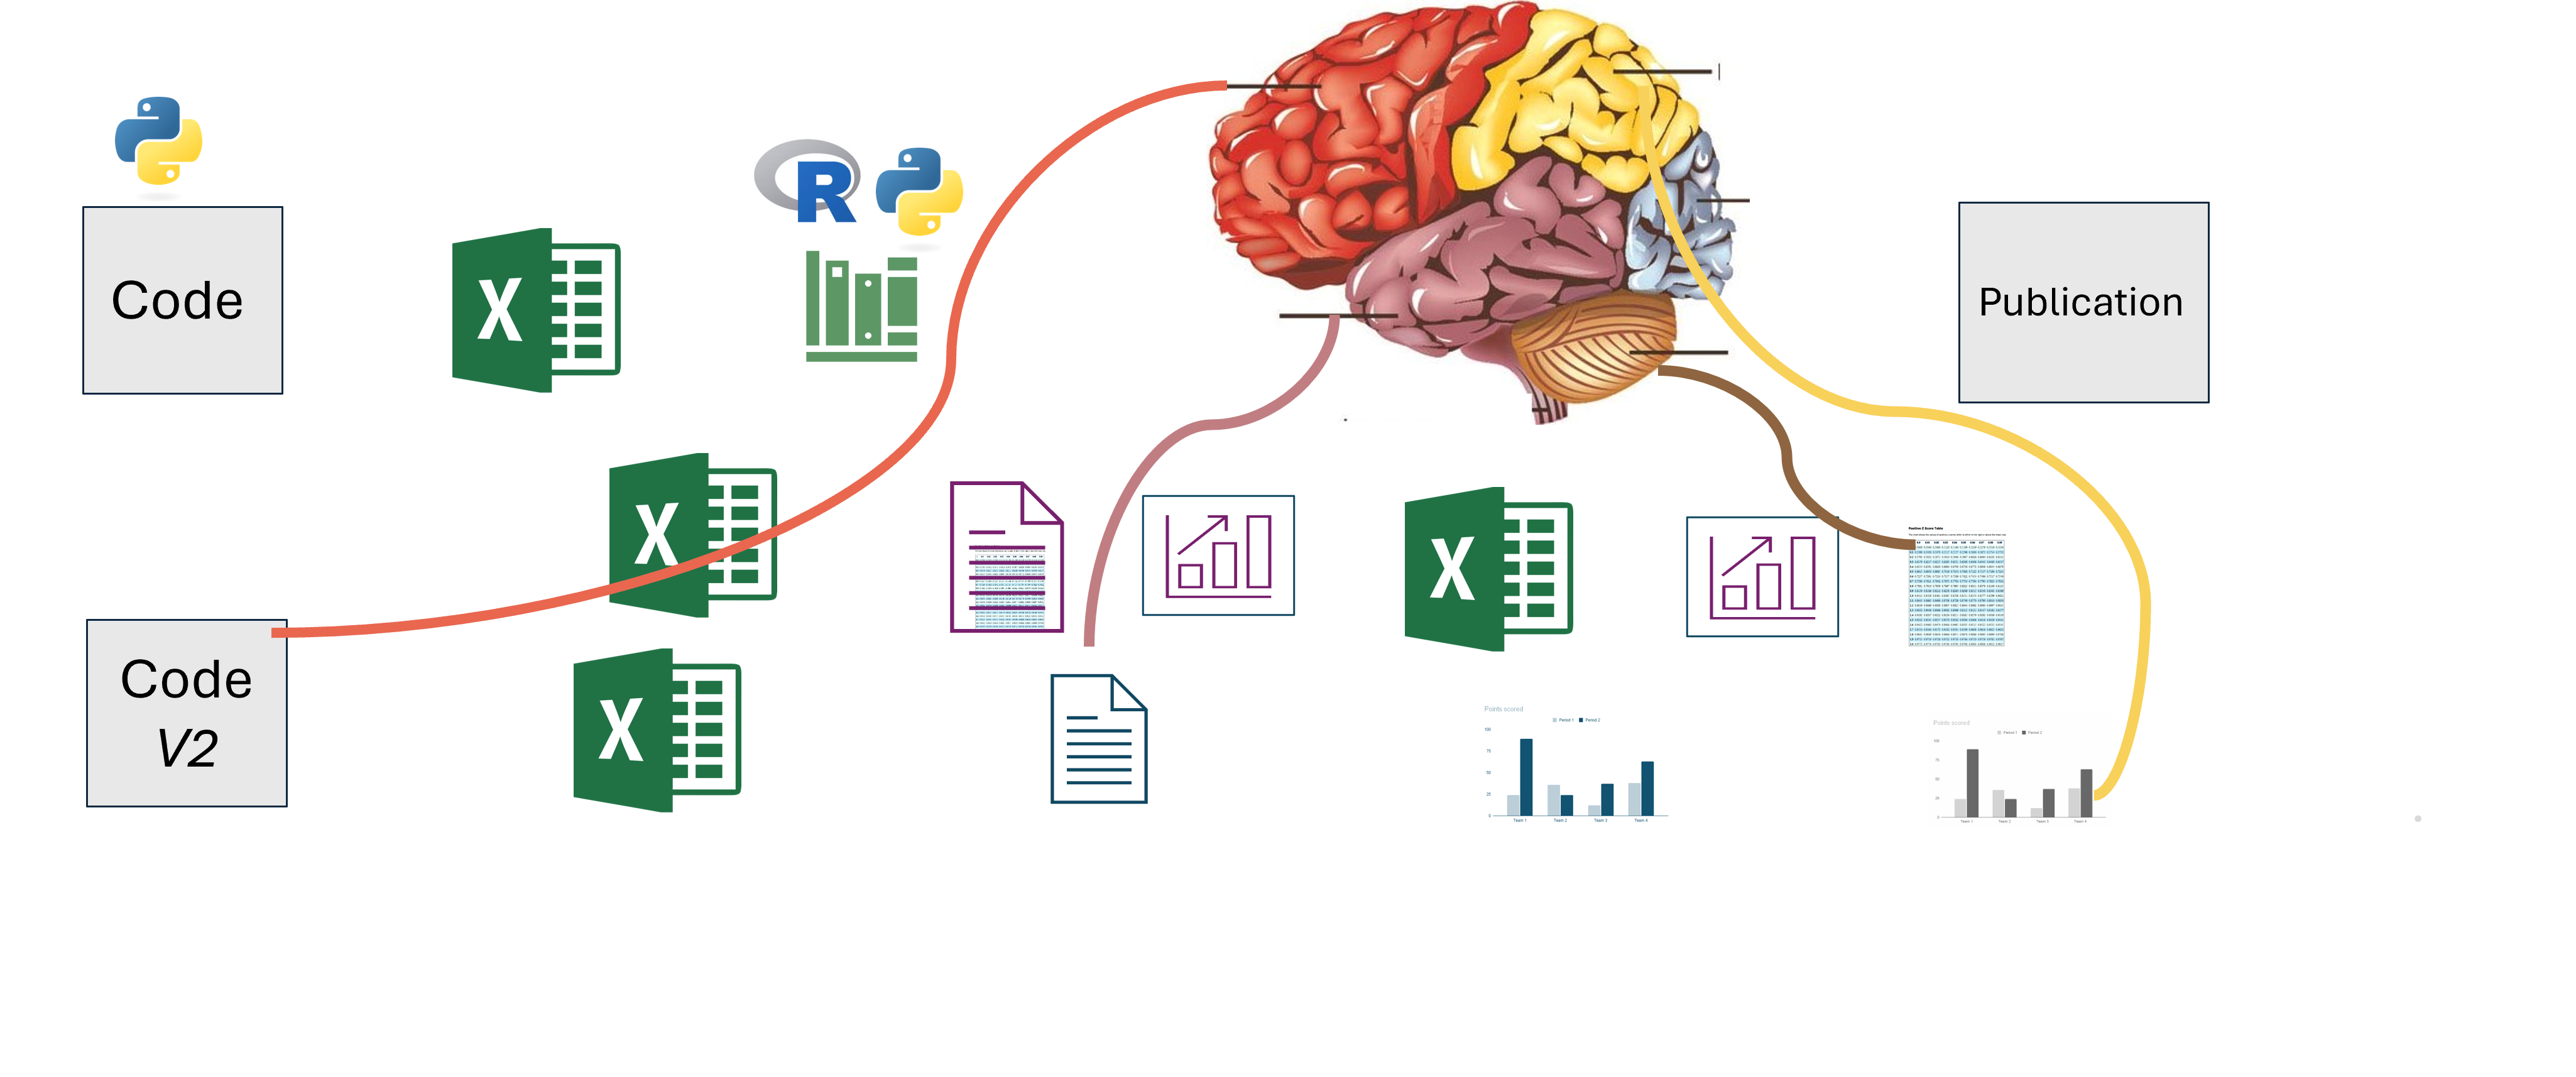
\includegraphics[width=1.0\textwidth]{Process18.png}}
        \only<7>{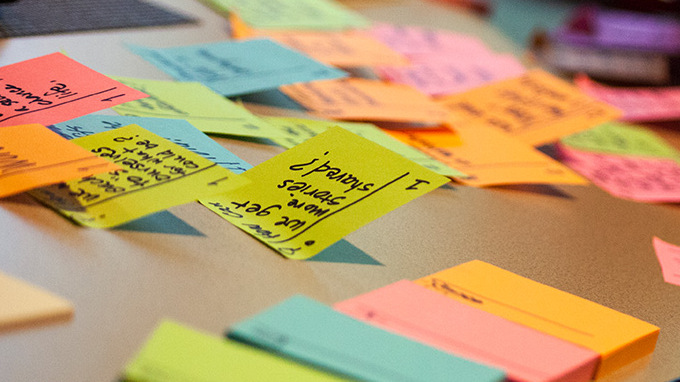
\includegraphics[width=1.0\textwidth]{Post-it.jpg} }
    \end{itemize}
    \end{column}
  \end{columns}
\end{frame}

\section{Issues}

\begin{frame}{What are the issues?}
  \begin{columns}[T]
    \begin{column}{0.5\textwidth}
      \begin{itemize}
        \item Errors due to cut and paste
        \item Errors are difficult to track
        \item Each operator has his/her own approach
        \item Several versions of code may coexist
        \item The steps aren't recorded
        \item Reproducibility is not granted
        \item Quality control is hard
      \end{itemize}
    \end{column}
    \begin{column}{0.5\textwidth}
      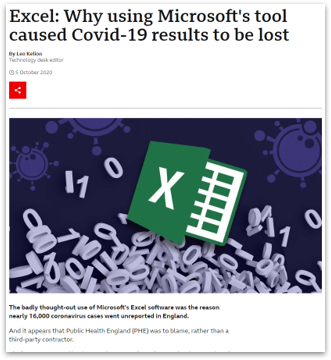
\includegraphics[width=0.8\textwidth]{ExcelUK.png}
    \end{column}
  \end{columns}
\end{frame}

% Other slides should go here...

\section{RAP}  % Better practices


\begin{frame}{What does a RAP look like?}
  \begin{columns}[T]
    \begin{column}{0.6\textwidth}
      \begin{itemize}
        \item It is a simple process:
          \begin{itemize}
            \item Linking inputs (data) to outputs (publication)
          \end{itemize}
      \end{itemize}
    \end{column}
    \begin{column}{0.4\textwidth}
      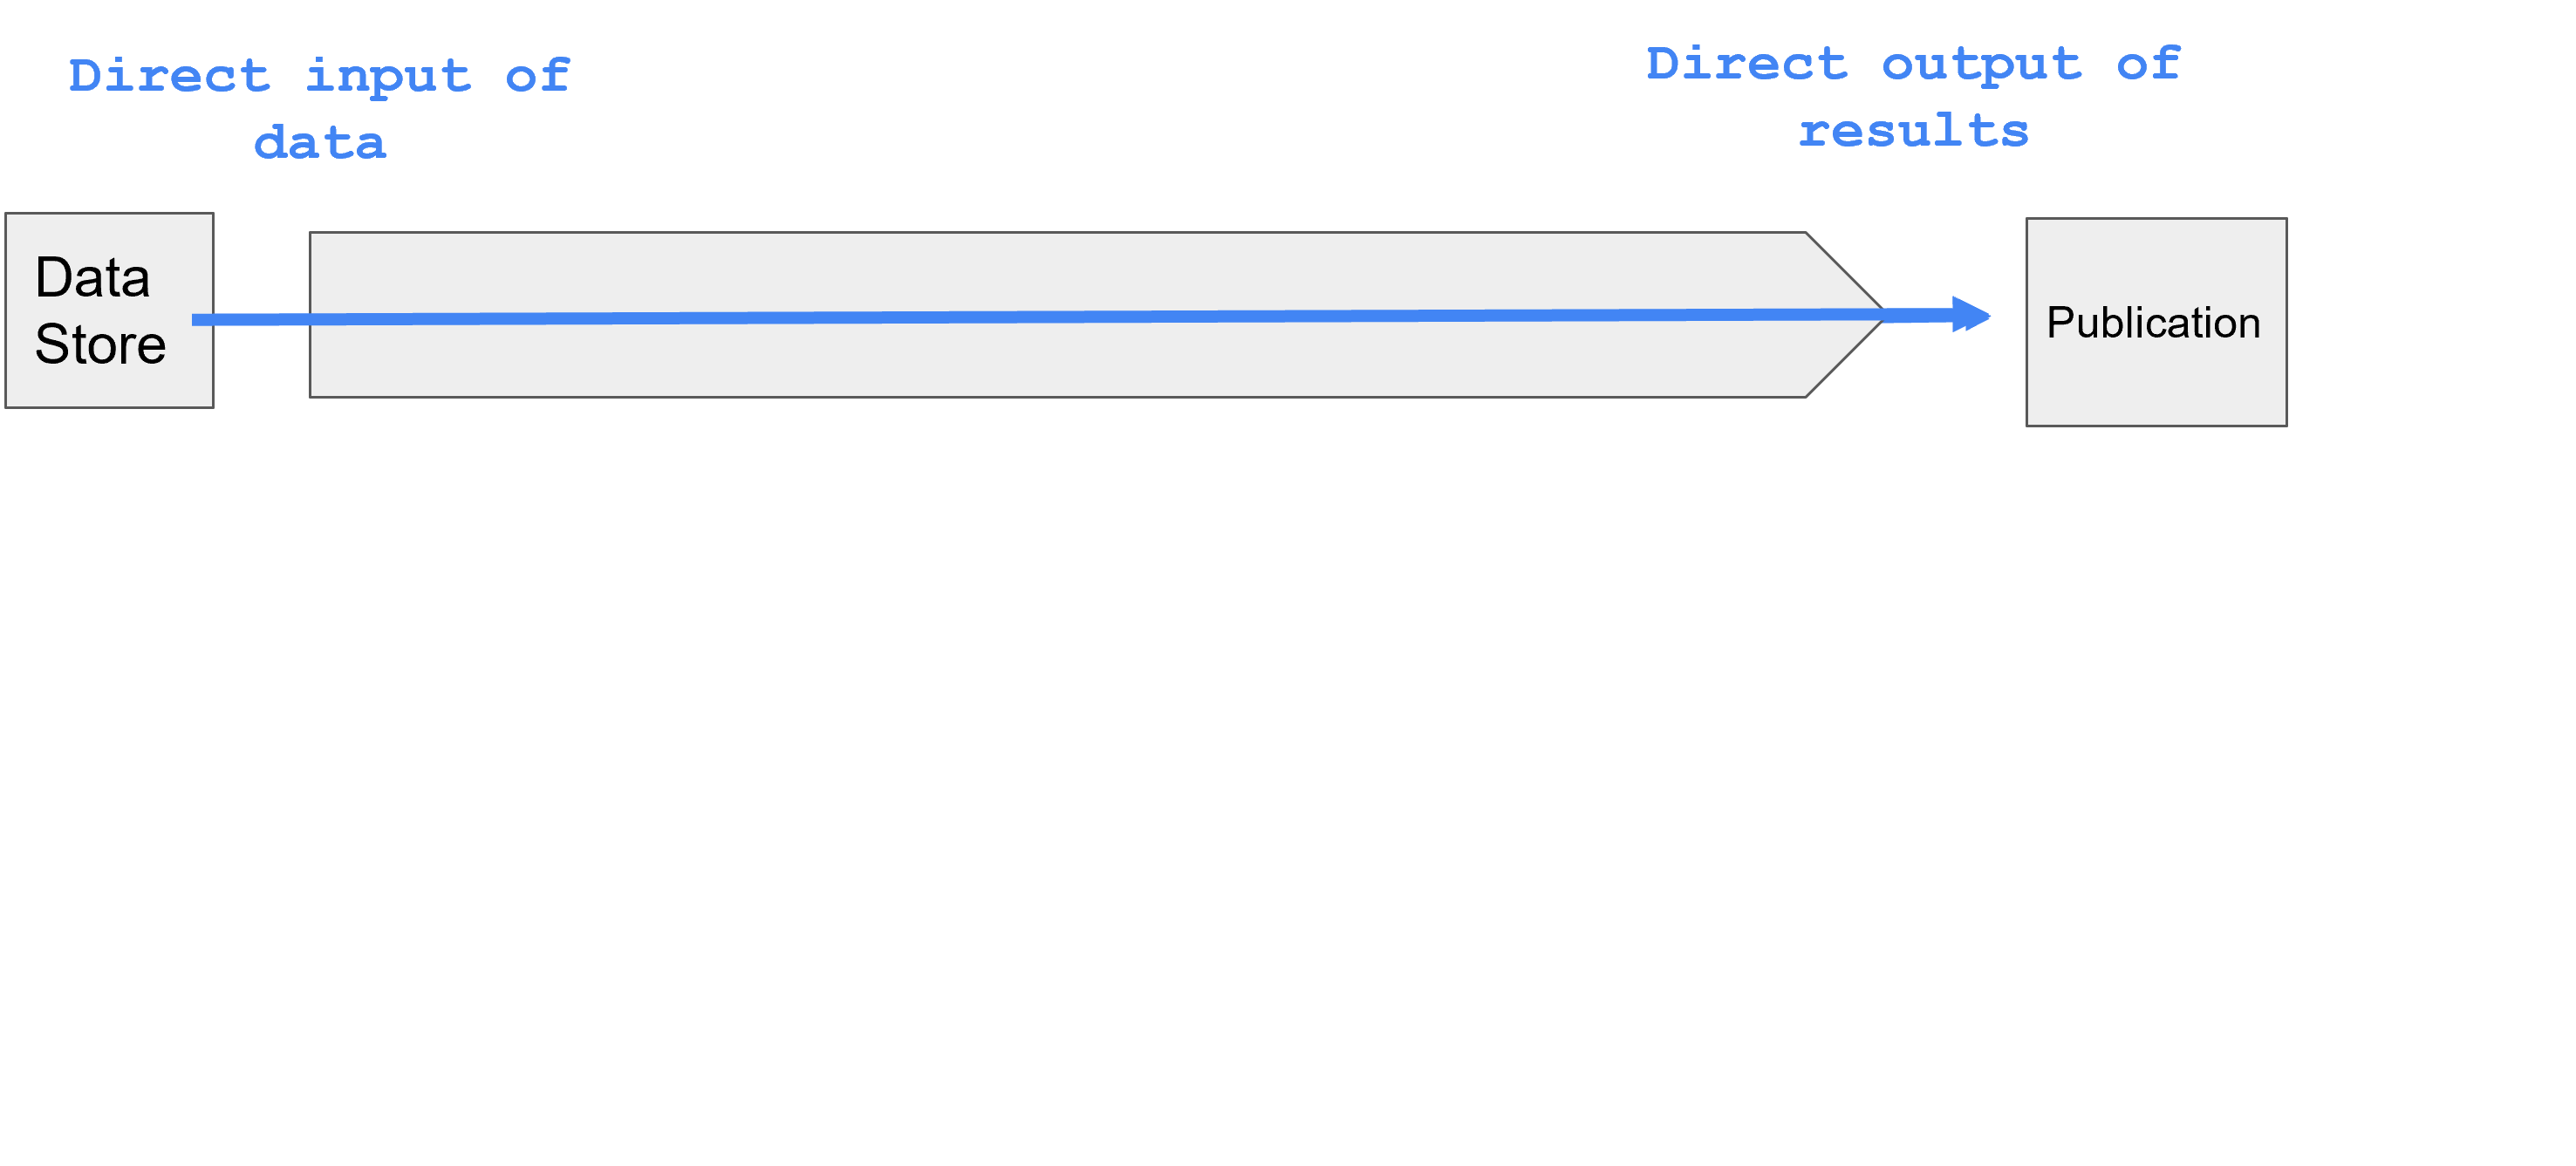
\includegraphics[width=\textwidth]{RAP-Pipeline1.png}
    \end{column}
  \end{columns}
\end{frame}

% Other slides go here...

\section{3 Principles}

\subsection{Examples}

\section{Version Control}


\begin{frame}{Useful resources}
  \begin{itemize}
    \item The UK government RAP \href{https://ukgovdatascience.github.io/rap-website/index.html}{website}.
    \item UK best practice \href{https://gss.civilservice.gov.uk/policy-store/quality-statistics-in-government/\#reproducible-analytical-pipelines-rap-}{documentation}.
    \item A free RAP \href{https://www.udemy.com/course/reproducible-analytical-pipelines/}{course} to teach you all you need to know.
    \item How the Data Science Campus sets its coding \href{https://datasciencecampus.github.io/coding-standards/}{standards}.
    \item A new open-source \href{https://the-turing-way.netlify.com}{book} from the Alan Turing institute setting out how to do reproducible data science.
  \end{itemize}
\end{frame}




\end{document}


